%\pdfoutput=1
% Uncomment line above if submitting to arXiv and using pdflatex

% $Id: main.tex 65869 2015-01-14 08:53:54Z pluca $
% ============================================================================
% Purpose: Template for LHCb documents
% Authors: Tomasz Skwarnicki, Roger Forty, Ulrik Egede
% Created on: 2010-09-24
% ============================================================================
\documentclass[12pt,a4paper]{article}
% For two column text, add "twocolumn" as an option to the document
% class. Also uncomment the two "onecolumn" and "twocolumn" lines
% around the title page below.

% Variables that controls behaviour
\usepackage{ifthen} % for conditional statements
\newboolean{pdflatex}
\setboolean{pdflatex}{true} % False for eps figures 

\newboolean{articletitles}
\setboolean{articletitles}{true} % False removes titles in references

\newboolean{uprightparticles}
\setboolean{uprightparticles}{false} %True for upright particle symbols

\newboolean{inbibliography}
\setboolean{inbibliography}{false} %True once you enter the bibliography

\input{preamble}
\usepackage{longtable} % only for template; not usually to be used in PAPERs

\usepackage{multirow}

\begin{document}

%%%%%%%%%%%%%%%%%%%%%%%%%
%%%%% Title     %%%%%%%%%
%%%%%%%%%%%%%%%%%%%%%%%%%
\renewcommand{\thefootnote}{\fnsymbol{footnote}}
\setcounter{footnote}{1}

% %%%%%%% CHOOSE TITLE PAGE--------
%\onecolumn
\input{title-LHCb-ANA}
%\input{title-LHCb-CONF}
%% $Id: title-LHCb-PAPER.tex 61931 2014-10-14 09:51:37Z roldeman $
% ===============================================================================
% Purpose: LHCb-PAPER journal paper title page template
% Author: 
% Created on: 2010-09-25
% ===============================================================================

%%%%%%%%%%%%%%%%%%%%%%%%%
%%%%%  TITLE PAGE  %%%%%%
%%%%%%%%%%%%%%%%%%%%%%%%%
\begin{titlepage}
\pagenumbering{roman}

% Header ---------------------------------------------------
\vspace*{-1.5cm}
\centerline{\large EUROPEAN ORGANIZATION FOR NUCLEAR RESEARCH (CERN)}
\vspace*{1.5cm}
\hspace*{-0.5cm}
\begin{tabular*}{\linewidth}{lc@{\extracolsep{\fill}}r}
\ifthenelse{\boolean{pdflatex}}% Logo format choice
{\vspace*{-2.7cm}\mbox{\!\!\!\includegraphics[width=.14\textwidth]{lhcb-logo.pdf}} & &}%
{\vspace*{-1.2cm}\mbox{\!\!\!\includegraphics[width=.12\textwidth]{lhcb-logo.eps}} & &}%
\\
 & & CERN-PH-EP-2015-078 \\  % ID 
 & & LHCb-PAPER-2015-009 \\  % ID 
 & & 23 March 2015  \\
\end{tabular*}

\vspace*{1.5cm}

% Title --------------------------------------------------
{\bf\boldmath\huge
\begin{center}
  Differential branching fraction
  and angular analysis of
  \decay{\Lb}{\Lz\mumu} decays
\end{center}
}


\vspace*{0.7cm}

% Authors -------------------------------------------------
\begin{center}
The LHCb collaboration\footnote{Authors are listed at the end of this paper.}
\end{center}

%\vspace{\fill}

% Abstract -----------------------------------------------
\begin{abstract}
  \noindent
  The differential branching fraction of the rare decay
  \decay{\Lb}{\Lz\mumu} is measured as a function of \qsq, the square
  of the dimuon invariant mass.  The analysis is performed using
  proton-proton collision data, corresponding to an integrated
  luminosity of 3.0\invfb, collected by the \lhcb experiment. 
  Evidence of signal is observed in the \qsq region below the square
  of the \jpsi mass. Integrating
  over $15 < \qsq < 20$ \gevgevcccc 
 the branching fraction
 is measured as
\begin{equation}
\deriv\BF(\decay{\Lb}{\Lz\mumu})/\deriv\qsq = (1.18 \;^{+\,0.09}_{-\,0.08} \pm 0.03 \pm 0.27 )
\times 10^{-7}\;(\gevgevcccc)^{-1},
\nonumber
\end{equation}
 \noindent where the uncertainties are statistical, 
 systematic and due to the normalisation mode,
 \decay{\Lb}{\jpsi\Lz}, respectively.
 In the \qsq\ intervals where the signal is observed, angular
 distributions are studied and the forward-backward asymmetries
 in the dimuon ($A_{\rm FB}^{\ell}$) and hadron ($A_{\rm FB}^{h})$ systems
 are measured for the first time.
 In the range $15 < \qsq < 20$ \gevgevcccc they are found to be
\begin{equation}
\begin{split}
A_{\rm FB}^{\ell} & = -0.05 \; \pm 0.09 \; \text{(stat)} \; \pm  0.03 \; \text{(syst)} \text{\;and} \\
A_{\rm FB}^{h} & = -0.29 \; \pm 0.07 \; \text{(stat)} \; \pm  0.03 \; \text{(syst)}.
\end{split}
\nonumber
\end{equation}

\end{abstract}

\vspace*{1.0cm}

\begin{center}
  Submitted to JHEP
\end{center}

\vspace{\fill}

{\footnotesize 
\centerline{\copyright~CERN on behalf of the \lhcb collaboration, licence \href{http://creativecommons.org/licenses/by/4.0/}{CC-BY-4.0}.}}
\vspace*{2mm}

\end{titlepage}


%%%%%%%%%%%%%%%%%%%%%%%%%%%%%%%%
%%%%%  EOD OF TITLE PAGE  %%%%%%
%%%%%%%%%%%%%%%%%%%%%%%%%%%%%%%%

%  empty page follows the title page ----
\newpage
\setcounter{page}{2}
\mbox{~}

\cleardoublepage








%\twocolumn
% %%%%%%%%%%%%% ---------

\renewcommand{\thefootnote}{\arabic{footnote}}
\setcounter{footnote}{0}

%%%%%%%%%%%%%%%%%%%%%%%%%%%%%%%%
%%%%%  Table of Content   %%%%%%
%%%%%%%%%%%%%%%%%%%%%%%%%%%%%%%%
%%%% Uncomment next 2 lines if desired
%\tableofcontents
%\cleardoublepage


%%%%%%%%%%%%%%%%%%%%%%%%%
%%%%% Main text %%%%%%%%%
%%%%%%%%%%%%%%%%%%%%%%%%%

\pagestyle{plain} % restore page numbers for the main text
\setcounter{page}{1}
\pagenumbering{arabic}

%% Uncomment during review phase. 
%% Comment before a final submission.
\linenumbers

% You can include short sections directly in the main tex file.
% However, for larger papers it is desirable to split the text into
% several semiautonomous files, which can be revised independently.
% This is especially useful when developing a document in
% collaboration with several people, since then different parts can be
% edited independently.  This type of file organization is shown here.
% 

\chapter{Testing lepton flavour universality with $R_{\Kstarz}$}
\label{sec:RKst_theory}

Lepton Flavour Universality (LFU) is the equality of the weak coupling constants for all leptons.
%and can be broken in NP scenarios. 
FCNC processes, which are forbidden in the SM at tree level and proceed only via loop diagrams,
are ideal to study LFU as new physics contributing in the loops could break the flavour symmetry.
 
In this work $b \rightarrow s\mumu (\ee)$ decays are studied to test LFU between electrons and muons. 
In particular, the \Bz meson semileptonic decays $\Bz\to\Kstarz\ll$ are considered.
Figure~\ref{fig:RKpenguins} shows the possible Feynman diagrams  producing such decays while 
Fig.~\ref{fig:NPpenguins} illustrates how these Feynman diagrams may include new particles. 
A series of recent LHCb measurements~\cite{TomRDreview} points to a tension with SM predictions, which makes
these processes particularly interesting as they can provide independent verifications of the existing discrepancy.
%
\begin{figure}[h]
\centering \includegraphics[width=0.8\textwidth]{RKst/figs/penguins3.png}
\caption{Loop diagrams producing $\Bz \to \Kstarz\ll$ decays.}
\label{fig:RKpenguins}
\end{figure}

In order to exploit the sensitivity of loop diagrams, in 2004 Hiller and Kruger proposed the measurement 
of the $R_H$ ratios~\cite{Hiller:2003js}, defined as
\begin{equation}
\label{eqRX}
R_{H} = \frac{\int_{\qsq_{min}}^{\qsq_{max}} \frac{ d\BR(\Bd \to H \mumu) }{\mathrm{d}\qsq}\mathrm{d}\qsq}{ \int_{\qsq_{min}}^{\qsq_{max}}\frac{ d\BR(\Bz \to H\epem) }{\mathrm{d}\qsq} \mathrm{d}\qsq} ,
\end{equation}
where $H$ can be an inclusive state containing an $s$ quark ($X_s$) or an $s$-quark resonance such as $K$ or $\Kstarz$.
In this quantity the differential branching fraction is integrated over the dilepton invariant mass squared, \qsq, from 
$\qsq_{min} = 4m_{\mu}^2$, which is the threshold for the $\mu\mu$ process, up to \mbox{$\qsq_{max} = (m_{\Bz} - m_H)^2$.} 

%The notation $\BR(X \rightarrow ~final ~state)$ denotes the fraction of $X$ particles which decays in the 
%given final state, this is called ``branching ratio". For example $\BR(\Bz\to\Kstar\mumu)$ is the
%fraction of \Bz particles which decays into $\Kstar\mumu$ with respect to all allowed \Bz decays.

The advantage of using ratios of branching fractions as observables is that, in the theoretical prediction, hadronic 
uncertainties cancel out. Furthermore, some of the experimental systematic uncertainties also approximately cancel in 
the ratios, improving the precision of the the measurement. For example, the measured quantities are the number of 
$\mu\mu$ and $ee$ decays recorded in a certain period of time. The luminosity, $\mathcal{L}$, is then used to obtain a
cross section, $\sigma$, using $R = \mathcal{L}\sigma$, where $R$ is the rate at which the decays occur. 
However, the luminosity measurement, usually a source of systematic uncertainty, appears on both
sides of the ratio and therefore cancels out.

\begin{figure}[h]
\centering \includegraphics[width=0.8\textwidth]{RKst/figs/penguins.png}
\caption{Example of penguin diagrams, on the left involving SM particles and on the right 
involving new possible particles.}
\label{fig:NPpenguins}
\end{figure}

Since the SM assumes lepton flavours universality, the predicted value of the ratio 
is $R_H = 1$, when the leptons are massless. Taking into account effects of order 
$m_\mu^2 / m_b^2$ Hiller and Kruger calculate that in the SM and in the full \qsq range~\cite{Hiller:2003js}:
%
\begin{align}
R_{X_s} = 0.987 \pm 0.006, \\
R_K = 1.0000 \pm 0.0001, \\
R_{\Kstarz} = 0.991 \pm 0.002; \\
\end{align}
%
\noindent
under the assumptions that:
%
\begin{itemize}
\item right-handed currents are negligible;
\item (pseudo-)scalar couplings are proportional to the lepton mass;
\item there are no CP-violating phases beyond the SM.
\end{itemize}

The measurement of the $R_H$ ratios is of particular interest after the recent
measurement of the branching fraction of the $\Bs\to\mumu$ decay~\cite{CMS:2014xfa}, 
where no evidence of new physics was found. In fact the quantities $(R_H - 1)$ and
$\BR(\Bs \to \mumu)$ remain proportional with
%
\begin{equation}
\frac{R_H - 1}{\BR(\Bs \to \mumu)} \sim 2 \cdot 10^{-5}.
\end{equation}
%
A joint measurement of these two quantities can give much information and constrain MFV models.
If $R_H = 1$ and $\BR(\Bs \to \mumu)$ is close to the SM prediction as it is measured to be at present, 
this will allow strong constraints to be established on extensions of the SM.
If instead $R_H > 1$ and the equation above is not verified, this would mean that one of the
assumptions listed above are not verified, which can happen is some extensions of the SM, such
as Super-symmetric models with broken R-parity.
%A series of recent LHCb measurements~\cite{TomRDreview} shows tensions with
%SM predictions, which makes it interesting to further investigate these processes.

\section{Combining ratios}

The full power of the $R_H$ ratios in understanding new physics scenarios comes from
their combinations.  In Ref.~\cite{Hiller:2014ula} Hiller and Schmaltz propose the measurement 
of the double ratios, $X_H = R_H / R_K$, which not only can test LFU but also allow
to disentangle the nature of the new physics that lies behind it. These ratios are in fact sensitive
to FCNCs of right-handed currents. Furthermore, in Ref.~\cite{Hiller:2014ula} the study is extended
to \Bs decays such as $\Bs\to\phi\ll$ and $\Bs\to\eta\ll$.

Parity and Lorentz invariance require that the Wilson Coefficients with left-handed chirality ($C$)
and their right-handed counterparts ($C'$) appear in the decay amplitude of exclusive decays in
specific combinations, \emph{e.g.}:
\begin{equation}
\begin{array}{ll}
C+C': & K, \Kstarz_{\perp}, ...  \\
C-C': & K_0(1430), \Kstarz_\parallel, ...
\end{array}
\end{equation}
where the labels for the \Kstarz meson represent its longitudinal (0), parallel $(\parallel)$ and
perpendicular $(\perp)$ transversity components. The $C$ contributions are universal for
all decays and therefore $X_H$ double ratios are sensitive to right-handed currents.
In fact the $R_H$ ratios can be expressed in terms of their deviation from unity as
\begin{equation}
\begin{array}{rl}
R_K \simeq 			& 1+ \Delta_+, 		\\
R_{K_0(1430)} \simeq 	& 1+ \Delta_-,		\\
R_{\Kstarz} \simeq 		& 1+ p(\Delta_- - \Delta_+) + \Delta_+,
\end{array}
\end{equation}
where the $\Delta_\pm$ quantities are combinations of Wilson coefficients
described in Eq.~10 of Ref.~\cite{Hiller:2014ula} and the parameter $p$ is the polarisation of \Kstarz
that in Ref.~\cite{Hiller:2014ula} is determined to be close to 1, simplifying the formula to $R_{\Kstarz} \simeq 1+ \Delta_-$.
In particular one can make the following observations: 
\begin{itemize}
\item $R_K < 1$, as it is measured to be, and $X_{\Kstarz} > 1$ points to dominant BSM contributions into $C_{LR}$ (see definition in Sec.~\ref{sec:operators});
\item a SM-like $R_K \sim 1$ together with $X_{\Kstarz} \neq 1$ requires BSM with $C_{LL} + C_{RL} \simeq 0$;
\item $R_K \neq 1$ and $X_{\Kstarz} \simeq 1$ corresponds to new physics in $C_{LL}$.
\end{itemize}

\section{Experimental status}

The $R_K$ and \RKst ratios have been measured at the B-factories~\cite{Lees:2012tva,Wei:2009zv},
while the recent measurement from LHCb~\cite{Aaij:2014ora} represents the most precise determination 
of $R_K$ to date; measured values are summarised in Tab.~\ref{tab:expstatus}.
The LHCb measurement manifests a $2.6~\sigma$ deviation from the SM prediction. This is particularly interesting as this
discrepancy can be explained with a new physics contribution in $C_9$ which also explains other existing tensions~\cite{Altmannshofer:2014rta,Descotes-Genon:2013wba,Hurth:2016fbr}.
It is also worth mentioning the measurement of the 
\mbox{$\mathcal{B}(\bar{B}^0 \to D^{*+}\tau^{-}\bar{\nu}_{\tau})/\mathcal{B}(\bar{B}^0 \to D^{*+}\mu^{-}\bar{\nu}_{\mu})$} 
ratio, which also probes LFU and was measured to be $2.1~\sigma$ larger than the value expected from the assumption 
of lepton universality in the SM~\cite{Aaij:2015yra}.
By profiting from the large dataset collected during Run-I, the LHCb experiment is expected 
to reduce the uncertainty on \RKst by at least a factor of 2 with respect to the B-factories.
%
\begin{table}[b]
\renewcommand\arraystretch{1.5}
\centering
\caption{Experimental status of the $R_{K^{(*)}}$ measurements. } %by the BaBar~\cite{Lees:2012tva} and Belle~\cite{Wei:2009zv} experiment.}
\begin{tabular}{$c|^c^c^c}
\rowstyle{\bfseries}
 Ratio	& Belle 			& BaBar 		& LHCb \\
 \hline
$R_K$			& $1.06 \pm 0.48 \pm 0.05$	& $1.38^{+0.39+0.06}_{-0.41-0.07}$ & $0.745^{+0.090}_{-0.074} \pm 0.036$\\
$R_{\Kstarz}$	& $0.93 \pm 0.46 \pm 0.12$	& $0.98^{+0.30+0.08}_{-0.31-0.08}$ & ---\\
\end{tabular}
\label{tab:expstatus}
\end{table}
\clearpage

\section{Analysis strategy}

The aim of the analysis in this chapter is to measure the $R_{\Kstarz}$ ratio using $pp$ collision data
collected by the LHCb detector in 2011 and 2012, corresponding to 3 \invfb of integrated luminosity.
The $\Bz \to \Kstarz\mumu$ and $\Bz \to \Kstarz\epem$, ``rare channels", are
reconstructed via the $\Kstarz$ decay into a kaon and a pion with opposite charges.

The analysis has to separate signal candidates from background candidates which have similar observed properties. 
The selection presented in Sec.~\ref{sec:RKst_selection} aims to maximise the yield while minimising
the background contamination. Two types of backgrounds are identified: ``peaking background" and ``combinatorial background". 
The first comes from misreconstructed or partially reconstructed decays. Due to its specific kinematic properties, this type 
of background usually peaks in some variable such as the invariant
mass of all final particles and, therefore, these candidates can be removed using specific cuts. 
In contrast, the combinatorial background arises from the random combination of particles and can 
be reduced by selecting candidates with good-quality tracks and vertices.

To further reduce the systematic uncertainties the measurement is performed as the double ratio 
%
\begin{equation}
\label{eq:RKst}
R_{\Kstarz} = 
\frac{N_{\Bz\to\Kstarz \mumu}}{N_{\Bz\to\Kstarz\jpsi\to \mumu}} 
\cdot \frac{N_{\Bz\to\Kstarz \jpsi \to \ee}}{N_{\Bz\to\Kstarz\ee}}
\cdot \frac{\varepsilon_{\Bz\to\Kstarz \jpsi \to \mumu}}{\varepsilon_{\Bz\to\Kstarz \mumu}} 
\cdot \frac{\varepsilon_{\Bz\to\Kstarz \ee}}{\varepsilon_{\Bz\to\Kstarz\jpsi\to \ee}},
\end{equation}
%
where decays reaching the same final states as the rare channels via a \jpsi resonance, $\Bz\to\Kstarz(\jpsi\to\ll)$,
also referred to as ``charmonium" or ``resonant" channels, are used as control samples.
These decays are distinguished from the rare channel using the invariant mass of the dilepton pair.
%
%In Sec.~\ref{sec:RKst_efficiency} the efficiency of selecting and reconstructing each channel is extracted
%and, finally, in Sec.~\ref{sec:RKst_result} the $R_{\Kstar}$ ratio defined is built as the double ratio
%of rare and resonant channels:
%
As new physics is not expected to affect tree level $b\to\cquark\cquarkbar\squark$ processes, the ratio 
between the \jpsi channels, $r_{\jpsi}$, \mbox{is 1} and therefore \mbox{$\RKst^{'} = \RKst \cdot r_{\jpsi} = \RKst$}.
On the other hand, using the relative efficiencies between the rare and resonant channels
causes many systematic effects to cancel resulting in a better control of systematic uncertainties.  

For brevity, the rare channels will also be denoted as ``$\ell\ell$", or
specifically ``$ee$'' and ``$\mu\mu$'', and the resonant channels as ``$\jpsi(\ell\ell)$'',
or ``$\jpsi(ee)$'' and ``$\jpsi(\mu\mu)$''.

\section{Dilepton invariant mass intervals}
\label{sec:RKst_q2_choice}

Three \qsq intervals are considered in this work: 
\begin{itemize}
\item the ``low-$q^2$" region, [0.0004,1.1]~\gevgevcccc, where the $\bquark\to\squark\ll$ process is dominated by the photon pole;
\item the ``central-$q^2$" region, [1.1,6.0]~\gevgevcccc;
\item the ``high-$q^2$"region, above 15~\gevgevcccc.
\end{itemize}
%
The central-\qsq region is the most interesting place to look for new physics. In fact, at low \qsq values, below 
1~\gevgevcccc~the photon pole dominates leaving little space for new physics to be found. %~\ref{sec:theo_qsq}.
The choice of the lower limit of the low-\qsq interval is driven by the need to reject the background due to the 
$\Bz\to\Kstarz\gamma$ decay where the photon converts into electrons in the material of the detector.
The lower bound of the central interval is set at 1.1~\gevgevcccc, to exclude a possible contribution from $\phi\to\ll$ decays, 
which can dilute new physics effects, while the upper bound is chosen to be sufficiently far away from the \jpsi radiative
tail where predictions are less cleanly defined. The 6 -- 15~\gevgevcccc~region is characterised by the presence
of the narrow peaks of the \jpsi and \psitwos resonances. The lower bound of the high-\qsq region, where
the signal in the electron channel is still unobserved, is chosen to be sufficiently far from the \psitwos resonance.
Rare and normalisation channels are selected according to the \qsq interval they fall into (for details see Sec.~\ref{sec:RKst_selection}).

\subsection{Control channels}
Beyond the normalisation channels, $\jpsi(ee)$ and $\jpsi(\mu\mu)$, additional control channels
are used to perform cross-checks and better constrain some of the background components
in the electron fit; in particular, \BdToKstGee, also denoted as ``$\gamma (ee)$", where the photon 
converts into an \ee pair in the detector material and \BdToKstPsiee, also denoted as ``$\psitwos(ee)$".
All of the normalisation and control channels are distinguished by the \qsq interval
they fall into. % (for details see Sec.~\ref{sec:RKst_selection}).

\section{Data samples and simulation}

%The analysis in this chapter is based on a dataset corresponding to 3~\invfb of integrated
%luminosity collected by the LHCb detector in 2011 and 2012.
Simulated samples are used to study the properties of backgrounds, determine efficiencies and to train
a multivariate classifier. The hard interactions are generated with \textsc{Pythia8}, hadronic particles
are decayed using \textsc{EvtGen} and, finally, propagated into the detector using \textsc{Geant4} and reconstructed
with the same software used for data. Samples are generated with both 2011 and 2012, magnet up and down
conditions and are combined in the appropriate proportions, according to the data integrated luminosities.
The next section describes the corrections applied to the simulation to ensure that it provides a good description of data.

%distributions of key valiables were compared between data and simulation and correction 
%In Table \ref{TabMC} are reported the MC samples used
%together with the number of generated events and the branching fractions of the simulated processes

\subsection{Data-simulation corrections}
\label{sec:RKst_mc_weighting}

Since the multivariate classifier training (see Sec.~\ref{sec:RKst_mva}) and the calculation
of most of the efficiency components (see Sec.~\ref{sec:RKst_efficiency}) are obtained from
the study of simulated events it is important to verify that the simulation provides a reliable 
description of data. Two areas where this agreement is particularly important are 
the kinematics of the final particles and the occupancy of the detector.
The kinematics of the decays is characterised by the transverse momentum spectrum of
the \Bz. Discrepancies in this distribution also cause the spectra of the final particles
to differ from data and hence affect the efficiency determination as its value often
depends on the momentum of the final particles.
The occupancy of the detector is relevant as it is correlated to the invariant mass shape of the signal
due to the addition of energy clusters in the electromagnetic calorimeter,
which affects the momenta of the electrons especially when bremsstrahlung photons are emitted before the magnet.
The hit multiplicity in the SPD detector is used as a proxy for the detector occupancy.

Since it is important that these quantities are well modelled, the simulation is
reweighted so that their distributions in data and simulation match.
The weight is calculated using resonant $\decay{\Bz}{\Kstarz(\jpsi\to\ll)}$ candidates, for which the signal peak
is already visible in data after pre-selection (see Sec.~\ref{sec:RKst_selection}). However, the data still includes
a high level of background and distributions cannot be directly compared.
The $_s\mathcal{P}$lot technique~\cite{sPlot} is used to statistically subtract the background from
data and obtain pure signal distributions using the invariant mass as the control variable.
%This method is based on an estimation
%od the signal and background densities based on a fit to a control variable where
%the two are well distinct, usually the invariant mass.
Figure~\ref{fig:RKst_sW_mass} shows fits to the 4-body invariant mass of candidates after pre-selection.
Data and simulation are then compared and the ratio between the two distributions is used to reweight
the simulation. The discrepancy in the SPD multiplicity is solved as a first step and then the \Bz transverse momentum 
distributions are compared in data and simulation reweighted to account for the SPD multiplicity.

Distributions of \Bz transverse momentum and SPD multiplicity are reported in Fig.~\ref{fig:b0pt_nSPD_distrib}
and ratios of these distributions, which are used to reweight the simulation, are reported in 
Fig.~\ref{fig:b0pt_nSPD_ratios}. The weights for the SPD multiplicity are calculated
separately for 2011 and 2012 events, because distributions are significantly different
in the two years. The binnings are chosen to have approximately 
the same number of events in each bin to limit fluctuations.
Further corrections are made by reweighting the simulation for PID efficiency using the
\verb!PIDCalib! package as described in Sec.~\ref{sec:RKst_pid_eff} and, finally, 
$ee$ samples are also reweighted for L0 trigger efficiency as described in Sec.~\ref{sec:RKst_trigger_eff}.
Weights are always applied throughout unless specified.
%Finally in Fig.~\ref{fig:mc_data_comparison} distributions of other variables are compared
%between data and reweighted Monte Carlo and show that a good agreement is achieved.

 \begin{figure}[h!]
\centering
%\includegraphics[width=0.48\textwidth]{RKst/figs/sW/KstJPsEE_log_fitAndRes.pdf}
\includegraphics[width=0.72\textwidth]{RKst/figs/sW/KstJPsMM_log.pdf}
\caption{Fitted 4-body invariant mass distribution of $\jpsi(\mu\mu)$ candidates 
after pre-selection used to obtain $_s\mathcal{W}$eights.}
\label{fig:RKst_sW_mass}
\end{figure}

\begin{figure}[h!]
\centering
\includegraphics[width=0.49\textwidth]{RKst/figs/nspd_12.pdf}
\includegraphics[width=0.49\textwidth]{RKst/figs/bpt.pdf}
\caption{Distributions of number of SPD hits (left) and \Bz transverse momentum (right) in data and simulation.}
\label{fig:b0pt_nSPD_distrib}
\end{figure}

\begin{figure}[h!]
\centering
\includegraphics[width=0.49\textwidth]{RKst/figs/nspd_w.pdf}
\includegraphics[width=0.49\textwidth]{RKst/figs/bpt_w.pdf}
\caption{ Ratios of simulated over real data distributions used to correct the simulation
as a function of the number of SPD hits (left) and the \Bz transverse momentum (right). }
\label{fig:b0pt_nSPD_ratios}
\end{figure}





\input{mc_weighting}

\chapter{Selection}
\label{sec:RKst_selection}

The selection process, described in the following subsections,
is divided into several steps. 
First of all events have to fall into the detector acceptance, produce hits and be selected
on the basis of quality features, such as $\chi^2$ of tracks and vertices, this stage is
called ``stripping". Secondly it is required that some specific trigger lines were fired by the events.
After the trigger and stripping requirements, cuts are applied to remove backgrounds
from specific decays. These first three steps are referred to as ``pre-selection". 

%In a second step we apply some cuts so remove specific backgrounds coming from other decays which are
%misreconstructed or partially reconstructed. 
The next step consists in the application of particle identification (PID) conditions which remove a good
part of misreconstructed background and clear the way for the last step where a neural network is used
to remove combinatorial background.
In order to minimise systematic uncertainties the same selection requirements are applied to the rare signal
candidates and on their relative charmonium channel, a part from the \qsq cuts which serve to 
distinguish them. In order to identify the $\Bz \to\Kstarz(\jpsi\to \mumu)$ channel a dilepton mass
interval of 100 \mevcc around the nominal \jpsi peak~\cite{PDG2014} is selected.
%, while a 100 \mevcc interval is used in the electron case.
For the electron resonant channel it is not possible
to use a narrow cut on the \qsq and 4-body $m(K\pi\epem)$ invariant mass distributions are characterised
by a long radiative tail at low masses due to bremsstrahlung radiation. Furthermore, a cut in \qsq also
distorts the 4-body mass distribution at low masses and it is important to be able to fit a 
wide mass range to constrain backgrounds. For these reasons the interval to select
$\Bz \to\Kstarz(\jpsi\to \epem)$ candidates is chosen to go as low as possible without overlapping with
the rare channel interval. The electron resonant channel is therefore selected in the interval
[6,11] \gevgevcccc. Figure~\ref{fig:2D_q2_B0mass} shows two-dimensional distributions
of \qsq versus the 4-body $m(K\pi\ell^+\ell^-)$ invariant mass for events which pass the full selection.
On these plots horizontal bands can be seen at the \qsq corresponding to the \jpsi and \psitwos resonances.
On the plot for muons it is also evident a vertical band which corresponds to rare decay of interest.

\begin{figure}[t!]
\centering 
\includegraphics[width=1.\textwidth]{RKst/figs/electron_B0jpsi2D_selected.pdf}
\includegraphics[width=1.\textwidth]{RKst/figs/muon_B0jpsi2D_selected.pdf}
\caption{Two-dimensional distributions of \qsq versus 4-body $m(K\pi\ell\ell)$
invariant mass for the electron (top) and muonic (bottom) channels in 2012 data.}
\label{fig:2D_q2_B0mass}
\end{figure}


\section{Trigger and Stripping }
\label{sec:RKst_trigstripping}

Events are triggered for the $\mu\mu$ and the $ee$ channels by the trigger lines
reported in Tab.~\ref{tab:RKst_triglines}, where the logical $and$ of L0, Hlt1 and Hlt2
lines is required and the logical $or$ of the lines on the same level. The candidates are
required to be triggered-on-signal (TOS) for most of the stages, namely
it is required for the particle which triggered to be one of the particles used to build the signal candidates.
Only for L0Global, used in the electron case, we require a trigger-independent-of-signal (TIS),
this is aimed to collect all the possible statistics for the electron channels, which are the most challenging.
The L0Muon trigger requires hits in the muon detector, while L0Electron and L0Hadron use information
from the calorimeters; Hlt1TrackAllL0 adds information from the trackers to the L0 candidates and
triggers if the L0 decision is confirmed; finally, Hlt2Topo[2,3]BodyBBDT uses a reconstruction 
of the event and a neural network trained on events with a specific topology in order to detect decays.
%More information about the muon triggers can be found at Sec.~\ref{sec:Lb_trigger}.

\begin{table}[h!]
\begin{center}
\caption{Summary of the trigger lines used to select the $\mu\mu$ and the $ee$ channels.
Where not explicitly indicated, the lines are required to be TOS.}
\begin{tabular}{c|c}
$\mu\mu$ candidates &  $ee$ candidates \\
\hline
	L0Muon		& L0Electron\\
				& L0Hadron\\
				& L0Global (TIS)\\
\hline
	Hlt1TrackAllL0				& Hlt1TrackAllL0 \\
	Hlt1TrackMuon				&	 \\
\hline
	Hlt2Topo[2,4]BodyBBDT 		& Hlt2Topo[2,4]BodyBBDT \\
	Hlt2TopoMu[2,4]BodyBBDT 	& Hlt2TopoE[2,4]BodyBBDT \\
	Hlt2DiMuonDetachedDecision	&							\\
\end{tabular}
\label{tab:RKst_triglines}
\end{center}
\end{table}

For the electron channels the L0 lines have different properties, therefore the analysis 
is performed separately for three categories of events, depending on the L0 trigger that fired 
them. These categories are defined to be exclusive in the following way:
%
\begin{itemize}
\item Events triggered by at least one of the electrons in the signal candidate (L0E): \\
{\centering \verb!L0Electron_TOS! }
\item Events triggered by at least one of the hadrons in the signal candidate and not by L0Electron (L0H): \\
{\centering \verb|L0Hadron_TOS && !L0Electron_TOS| }
\item Events triggered by particles not in the signal candidate (Trigger Independent of Signal, TIS) and not by the previous cases (L0I): \\
{\centering \verb|L0_TIS && !(L0Electron_TOS |\verb!|| L0Hadron_TOS)! }
\end{itemize}

The majority of the selected events falls in the L0Electron category.
The L0Hadron category is more efficient at low \qsq were the \Kstarz has more momentum.

Candidates are then required to pass the kinematic and quality cuts summarised in Tab.~\ref{tab:RKstripping}. 
The meaning of variables in the table was already explained in Sec.~\ref{sec:Lb_selection}.
Loose PID cuts are applied in preselection to limit the size of the samples, while tighter cuts are applied
in a second stage. A large mass window is kept around the \Bz peak in order to be able
to fit the sideband and to train the multivariate analysis and constrain backgrounds.
%
%In the table $IP_{\chi_2}$ is defined as the projected distance from the vertex divided by its uncertainty, for example $IP^B_{\chi_2}(primary) > 4$ means
%that the B vertex is 2 standard deviations away from the primary vertex.
%Another quantity used is a pointing variable defined as the angle between the direction of the particle momentum and the flight direction from its mother vertex, called DIRA.
%This allows the selection of particles with well-defined primary vertices.
%%$GhostProb$ is the probability, estimated from the reconstruction algorithm, for the track to be a ghost. 
%Loose PID cuts are applied in preselection to limit the size of the samples, while tighter cuts are applied
%in a second stage. To quantify the PID of a particle the pion is used as a reference point and a Log-Likelihood
%variable is used. Therefore the {\verb PID } variable reported in the table is given in terms of the difference between
%the Log-Likelihood of the particle of a given type and a pion. This is called Delta Log-Likelihood (DLL).
%For example:
%\begin{equation}
%\verb!PID!_K = \text{DLL}_{K-\pi} = \log(\mathcal{L}_K) - \log(\mathcal{L}_\pi)
%\end{equation}
%
\begin{table}[]
\begin{center}
\caption{Summary of stripping cuts used for the central and high \qsq regions. }
\begin{tabular}{|c|c|}
\hline
Particle &  Cuts \\
\hline
%\multirow{2}{*}{ All final}
%       			&   track $\chi_2/\text{ndf} < 3$ \\
%       			&   {\verb GhostProb } $< 0.4$ \\
%\hline
$\pi$			& $\chisqip(primary) > 9$ \\      			
\hline
\multirow{3}{*}{K}
      			& {\verb PID }$_K > -5$ \\
       			& $\chisqip(primary) > 9$ \\
       			& {\verb hasRICH }  \\
 \hline
\multirow{4}{*}{ \Kstarz }
       			& $\pt > 500$ \mevc \\
       			& $|m - m_{\Kstarz}^{PDG}| < 100$ \mevcc  \\ %300 in stripping but then we restrict it to 100
       			& $\chisqip(primary) > 9$ \\
       			& Origin vertex $\chi_2/\text{ndf} < 25$ \\
\hline
\multirow{3}{*}{ $\mu$ }
       			& $\pt > 300$ \mevc \\
       			& $\chisqip(primary) > 9$ \\
       			& i{\verb sMuon }\\  %RequiresDet='MUON'
%       		& hasMuon \\
\hline
\multirow{4}{*}{ $e$ }
       			& $\pt > 300$ \mevc \\
       			& $\chisqip(primary) > 9$ \\
       			& {\verb hasCalo }\\ %RequiresDet='CALO'
       			& $PID_e > 0$ \\
\hline
\multirow{4}{*}{ Dilepton }
				& $m_{\ell\ell} < 5500$ \mevcc \\
			  	& End vertex $\chi^2/\text{ndf} < 9$ \\
			  	& Origin vertex $\chi^2$ separation $> 16$ \\
%			  	& $\chisqip(primary) > 0$ \\
\hline
\multirow{4}{*}{ $B^0$  }
 %      & $| m - m_{B^0}^{PDG}| < 600$ \mevcc  \\
       			& {\verb DIRA } $> 0.9995$ \\ 
       			& End vertex $\chi^2/\text{ndf} < 9$ \\
     			& $\chisqip(primary) < 25$ \\
     			& Primary vertex $\chi^2$ separation $> 100$ \\
\hline
\end{tabular}
\label{tab:RKstripping}
\end{center}
\end{table}
%
Track-quality and vertex quality cuts are also applied using the $\chi^2_{track}/\text{ndf}$, 
{\verb GhostProb }, and $\chi^2_{vtx}/\text{ndf}$
variables. The {\verb GhostProb } quantity describes the probability of a track being fake.
By construction cutting at 0.4 removes $(1 - 0.4)\cdot 100 = 60\%$ of fake tracks.
For details about the definition of the variables used see Ref.~\cite{Loki_twiki}.

\section{PID}
\label{sec:PID}

After preselection there still are high levels of misreconstructed background.
In particular, as the ID of kaons and pions are not constrained, the samples
still contain both ID combinations for most candidates, therefore tighter PID cuts are applied.
In the LHCb analysis framework the particle identification probability can be quantified
using the ``{\verb ProbNN }" variables~\cite{ProbNNs_pres}. These variables are the output
of a Neural Network which takes as input information from the calorimeters, the RICH detectors
and the muon system. Unlike the DLL variables these are bounded from 0 to 1 and can be
therefore directly be interpreted as probabilities.
For example {\verb ProbNNk } is the probability for a reconstructed particle to be a kaon.
Two tunes of the {\verb ProbNN } variables, labelled V2 and V3, are available.
Tune V3 was shown to be optimal for positive ID, while tune V3 was found to be optimal
for background rejection and therefore it is used to quantify the mis-ID probability.
%
\begin{figure}[h!]
\centering 
\includegraphics[width=0.48\textwidth]{RKst/figs/muon_PID.pdf}
\includegraphics[width=0.48\textwidth]{RKst/figs/electron_PID.pdf}
\caption{Correct ID probability distributions for muons (left)
and electron (right) in 2012 data.}
\label{fig:e_mu_pid}
\end{figure}
%
\begin{figure}[h!]
\centering 
\includegraphics[width=0.48\textwidth]{RKst/figs/kaon_PID.pdf}
\includegraphics[width=0.48\textwidth]{RKst/figs/pion_PID.pdf}
\caption{On the horizontal axis of these plots is shown the correct ID
probabilities for kaons (left) and pions (right), while the vertical
axis show the mis-ID probability.}
\label{fig:k_pi_pid}
\end{figure}

Figure \ref{fig:e_mu_pid} shows distributions of the correct ID variables
in the 2012 data sample while Fig.~\ref{fig:k_pi_pid} shows in a two-dimensional
plane the probability of correct identification and mis-identification of kaons and pions.
These plots are characterised by clear peak at maximal ID probability and minimal mis-ID
probability, corresponding to particles to which is possible to assign a well
defined identification.

In order to maximise the power of the PID cuts probabilities of correct ID 
and mis-ID are combined using the following cuts:
%
\begin{center}
\begin{tabular}{lcl}
$\pi$ &\to  & $\verb!ProbNNpi-V3! \times (1 - \verb!ProbNNk-V2!) \times (1 - \verb!ProbNNp-V2!) > 0.1$ \\
$K$   &\to  & $\verb!ProbNNk-V3! \times (1 - \verb!ProbNNp-V2! ) > 0.05$ \\ 
$\mu$ &\to  & $\text{min}(\verb! ProbNNmu-V3! , \verb! ProbNNmu-V3 !) > 0.2$  \\
$e$   &\to  & $\text{min}(\verb! ProbNNe-V3! , \verb! ProbNNe-V3 !) > 0.2$ \\
\end{tabular}
\end{center}
%
In the first formula, for example, {\verb ProbNNpi } is the probability of correctly identifying the
pion as a pion, while {\verb ProbNNk } is the probability of mistaking it for a kaon.
Therefore by maximising the quantity ``{\verb ProbNNpi } $\times$ (1 - {\verb ProbNNk })",
one can maximise the correct ID probability and minimise at the same time the mis-ID probability.
%In the kaon case we do not use requirements on the $K\to\pi$ mis-ID probability
%because this cut was found to be unacceptably inefficient.


\section{Peaking backgrounds }

Cuts are applied in order to remove background sources due to specific decays.
These types of backgrounds usually peak in some variable because of their mass
or distinctive kinematic properties and therefore they can be removed without significant
signal efficiency loss. In the following sections are described the main sources of peaking background.

\subsection{Charmonium vetoes}

Charmonium resonances such as \jpsi and \psitwos peak in \qsq.
The choice of \qsq binning described in Sec.~\ref{sec:RKst_q2_choice}
constitutes a natural veto for these decays. Simulated events were used
to check if resonant events leak inside the \qsq intervals chosen for
the rare channel analysis. For the muonic channels the leakage is negligible
as the peaks are sharper due to a better resolution and muons emit fewer
bremsstrahlung photons, resulting in shorter radiative tails.
The electronic channels are instead  characterised by
a worse resolution and at the same time electrons can radiate 
several bremsstrahlung photons, yielding long tails at low \qsq.
Analysing Monte Carlo events it was found that 1.3--2\% (depending on
the trigger category) of $\Bz\to\Kstar(\jpsi\to\ee)$ candidates leak into the $1.1 < \qsq < 6$
\gevgevcccc interval and 1.8\% of \psitwos events leak above 15 \gevgevcccc.
The contribution from these candidates is modelled in the fit. 


\subsection{$\phi$ veto}

It can happen that a kaon from the decay $B_s \rightarrow \phi \ell^+\ell^-$, where the $\phi$ decays in two kaons,
is mis-identified as a pion and therefore causes the $\phi$ to be reconstructed as a $\Kstarz$. This results in
a candidate with a value of $m_{K\pi}$ that is less than $m_{\Kstarz}$ but still high enough to
pass the selection requirements. In Fig.~\ref{fig:phiplots} is reported the plot of $m(K\pi)$ versus
$m(K\pi \ell\ell)$, where kaon mass hypothesis is assigned to the pion. A peak can clearly be seen
around the $\phi$ mass (1020 \mevcc).
To remove this background only candidates with $m_{K(\pi\rightarrow K)} > 1040$ \mevcc) are selected.
This results in a 98\% background rejection while keeping a 99\% signal efficiency.
%This cut could be further optimised using PID information. On the other hand LHCb simulation 
%struggles modelling the PID variables correctly. Therefore using PID in these cuts would
%add systematic uncertainties without significantly improving the signal efficiency which is already 99\%.
The $\phi$ could also constitute a background when it decays into two leptons but the
branching ratio of this decay is small compared to the one into kaons and this
contribution is taken into account by the choice of the \qsq intervals.

\begin{center}
\begin{figure}[h!]
\centering 
\includegraphics[width=0.48\textwidth]{RKst/figs/RKst/phi.pdf}
\includegraphics[width=0.48\textwidth]{RKst/figs/RKst/Kmumu.pdf}
\caption{ On the left the distribution of 2011 data events on the variables $(m_{K(\pi\rightarrow K)})$ 
and $(m_{K(\pi\rightarrow K)\mu\mu})$, where $\pi\rightarrow K$ means that the kaon mass is given 
to the pions too. On the right the mass of the three-body system $(m_{K\mu\mu})$
where the peak due to the $B^+ \rightarrow K^+ \mu\mu$ decay is visible. }
\label{fig:phiplots}
\end{figure}
\end{center}


\subsection{$\Bu \to K^+ \ll$ plus a random pion}

Some $\Bu \to K^+ \ell^+\ell^-$ decays can contaminate the upper \Bz mass sideband if they are combined
with a soft pion from somewhere else in the event and therefore reconstructed as a \Bz decay.
The same can also happen with a kaon misidentified as a pion combined with an other kaon in the event.
In Fig.~\ref{fig:phiplots} the invariant mass distribution of the three-body $K\mumu$ system, $m_{K\mu\mu}$, is shown.
This is characterised by a narrow peak at the $\Bu$ mass. Since these
candidates have $m_{K\pi\ell\ell} > 5380$ \mevcc  there is no contribution under the \Bz peak,
but they can cause problems when using sidebands events to train the neural network.
An effective veto for this decay was found to be max$(m_{K\ell\ell},m_{K\to\pi\ell\ell}) < 5100 ~\mbox{MeV/c}^2$,
which results in 95\% background rejection while keeping 99\% signal efficiency.

\subsection{$\Lambda_b$ decays}

\Lb\to\Lz\jpsi decays are unlikely to be reconstructed as $\Bz \to \Kstarz \ll$ because
the \Lz is long-lived and decays further in the detector with a separate vertex.
Simulated events were used to check how many candidates fall into the \Bz samples, which results to be negligible. 
The $\Lb\to\jpsi pK$ decay can instead contribute more easily since the $m(pK)$ is above the \Lz threshold
and therefore they must come from $\Lz^*$ resonances, which are not long-lived. This background is already
reduced using PID but a non-negligible contribution is still expected in the $\mu\mu$ sample, which is modelled in the fit.

\subsubsection{Other peaking backgrounds}

A possible background could come from $\Bz \to\Kstar\gamma$ decays where the photon converts
into two electrons while traversing the detector. In LHCb, around 40\% of photons convert before the calorimeter,
but only a small fraction of these, $\sim 10\%$, are reconstructed. Furthermore these events fall
into a \qsq region well below the intervals considered in these analysis and their contribution is therefore negligible.
Similar decays are also $\Bz \to\Kstar\eta$ and $\Bz \to\Kstar\pi^0$ where $\eta$ and the pion decay into
two photons. Once again the contribution from these decays falls well below the considered \qsq intervals.
Finally, a potentially dangerous background could come from events where the
identity of the kaon and the pion are swapped as these candidates peak under the signal.
Their contribution is found to be small, 0.5\%, however the effect of their modelling into the fit
is taken into account in the systematic uncertainties.

\subsection{Mis-reconstructed background}
\label{sec:RKst_peaking_Dchains}

A source of mis-reconstructed background is due to cascade decays with a \Bz decaying semileptonically
into a $D$ meson which also decays semileptonically, e.g. $\Bz\to D^{-} \ell^+ \bar{\nu_\ell}$
followed by $D^{-} \to \Kstarz \ell^- \nu_\ell$. The candidates built from these decays tend to have a low
4-body invariant mass as two or more particles are not reconstructed.
%This is in general true for any partially reconstructed background from $B$ decays.

In order to remove this background in the muonic channels, the 4-body $m(K\pi\mumu)$ invariant mass is recalculated
with a kinematical fit using the \verb!DecayTreeFitter! package. In the resonant case this includes a constraint of the dilepton
mass to be the \jpsi nominal mass and in both rare and resonant cases each particles is constrained to point to 
its origin vertex. This constraint has the effect of pushing the misreconstructed events far from the \Bz peak.
Therefore, to avoid this background, it is sufficient to limit the analysis to 4-body invariant masses
above 5150 \mevcc.

In the electron case it is instead important to fit a wider mass window to correctly constrain the background
therefore one cannot eliminate this mis-reconstructed background which is then modelled in the fit
(for details see Sec.~\ref{sec:RKst_misreco_fit}).


\section{Multivariate analysis}
\label{sec:RKst_mva}

The final selection is performed using a Neural Network classifier (NN) based on the NeuroBayes
package~\cite{Feindt:2006pm,feindt-2004}. The multivariate analysis is intended to remove
some combinatorial background and obtain a clearer signal peak.

For the final selection in the central and high \qsq intervals a Neural Network classifier (NN)
is used based on the NeuroBayes package \cite{Feindt:2006pm,feindt-2004}.
Representative samples of the signal and background are needed to train the classifier.
For the signal, fully reconstructed \BdToKstmm and \BdKstee simulated events can be used.
%The simulation is corrected improve the data-simulation agreement as described in (see Sec. \ref{sec:RKst_mc_weighting}).
A sample representative of the background can be obtained taking real data events
in the upper \Bz sideband: ($m(K\pi\mumu) > 5400$ \mevcc and $m(K\pi\ee) > 5600$ \mevcc). The lower sideband is not
used in the training as it contains a significant fraction of mis-reconstructed background.
All pre-selection cuts are applied to the background samples used for the training.
As L0 and PID variables are not well described these cuts are not applied in the Monte Carlo
samples but their effect is taken into account by the event weight.
To train the classifier 50\% of the sideband events was used, keeping the other 50\% for testing.
For the signal sample a number of Monte Carlo events was used equal to the number available for
the background sample. 

The input to the NN consists of 22 variables containing information about the kinematic of the decays
and the quality of tracks and vertices. All the variables used are listed in Tab.~\ref{tab:RKst_mva_vars}.
The graphical representation of the correlation matrices are shown in Fig.~\ref{fig:Rkst_nnCorrelation},
in these figures the variable with ID = 1 is the NN output and the other IDs are reported in Tab.~\ref{tab:RKst_mva_vars}.
%
The single most discriminating variable used is the $\chi^2$ of a kinematic fit
that constrains the decay product of the \Bz, the \Kstar and the dimuon, to originate from their respective vertices.
Other variables that contribute significantly are the $\chi^2_{IP}$ of \jpsi and \Kstar, the transverse momentum
of the \Bz and the pointing direction (DIRA) of the reconstructed \Bz to the primary vertex.
The list the 10 most important variables is reported in Tab.~\ref{tab:RKst_nnInputs}, together
with information on the relative importance of each input. The meaning of the column headings
in this table was already explained in Sec.~\ref{sec:Lb_mva}.

\begin{table}
\centering
\begin{tabular}{l|l}
Particle 	& Variables \\ \hline
\Bz			& $\chi^2_{DTF}/\text{ndf}$ [1], DIRA [19], $\chi^2_{FD}$ [15], $\chi^2_{vtx}/\text{ndf}$ [12], \chisqip [14], \pt [7] \\
\Kstar		& $\chi^2_{FD}$ [21], $\chi^2_{vtx}/\text{ndf}$ [11], \chisqip [2], \pt [5] \\
Dilepton	& $\chi^2_{FD}$ [17], $\chi^2_{vtx}/\text{ndf}$ [13], \chisqip [20], \pt [6] \\
$e$			& \chisqip [3][4], \pt [9][10]\\
$\mu$		& \chisqip [14][15], \pt [9][10]\\
K			& \chisqip [18], \pt [16]\\
$\pi$		& \chisqip [22], \pt [8]\\
\end{tabular}
\caption{Variables used as inputs for the NN training.
Next to each variable the ID number in brackets provides the index
reported in the correlation matrices shown in Fig.~\ref{fig:Rkst_nnCorrelation}.
}
\label{tab:RKst_mva_vars}
\end{table}

\begin{table}
\centering
\caption{Summary of inputs to the neural network in order of importance. The 10 most discriminating variables are shown.
Column ``adds'' gives correlation significance added by given input when adding it to list of those
ranked above, ``only this'' provides power of given input alone and ``loss'' shows how much information
is lost when removing only given input. Decay Tree Fit is performed using DecayTreeFitter tool
on whole decay chain with constraining tracks to appropriate vertex topology and the $m(p\pi)$
invariant mass to the PDG value.}
\begin{tabular}{|c|ccc|c|ccc|}\hline
\multicolumn{4}{|c|}{Muons} 														& \multicolumn{4}{c|}{Electrons}						  \\ \hline   
Input                   			& Adds 			& Only this 	& Loss 			& Input        							& Adds      & Only this & Loss    \\ \hline
$ \Bz$ $\chi^2_{DTF}/\text{ndf} $		& 80.44 		& 80.44 		& 13.14  		&	$ \Bz$ $\chi^2_{DTF}/\text{ndf} $		& 28.70 		& 28.70 		& 3.94  \\
$ \Kstar$ $\chisqip $		& 22.26 		& 67.58 		& 3.48  		&	$ \Kstar$ $\chisqip $		& 12.71 		& 25.11 		& 1.57  \\
$ \Bz\text{DIRA} $		& 10.58 		& 71.24 		& 3.95  		&	$ e_{2}$ $\chisqip $		& 6.56 		& 20.19 		& 3.30  \\
$ \Kstar$ $\pt $		& 9.16 		& 49.13 		& 2.07  		&	$ e_{1}$ $\chisqip $		& 5.54 		& 19.66 		& 2.60  \\
$ \jpsi$ $\chisqip $		& 6.58 		& 56.15 		& 1.35  		&	$ \Kstar$ $\pt $		& 3.74 		& 15.35 		& 3.14  \\
$ \Bz$ $\pt $		& 6.00 		& 41.42 		& 4.39  		&	$ \jpsi$ $\pt $		& 4.81 		& 5.55 		& 3.18  \\
$ \mu_{1}$ $\pt $		& 2.96 		& 15.85 		& 3.79  		&	$ \Bz$ $\pt $		& 2.78 		& 13.01 		& 2.20  \\
$ \mu_{2}$ $\pt $		& 2.73 		& 15.04 		& 3.46  		&	$ \pi$ $\pt $		& 3.08 		& 7.93 		& 1.83  \\
$ \jpsi$ $\pt $		& 3.06 		& 16.41 		& 2.84  		&	$ e_{2}$ $\pt $		& 2.35 		& 9.81 		& 2.74  \\
$ \Kstar$ $\chi^2_{vtx}/\text{ndf} $		& 2.41 		& 28.14 		& 2.38  		&	$ e_{1}$ $\pt $		& 2.15 		& 8.04 		& 2.28  \\

%$ \Bz$ $\chi^2_{FD} $		& 2.03 		& 63.73 		& 1.37  		&	$ \Kstar$ $\chi^2_{vtx}/\text{ndf} $		& 1.75 		& 7.45 		& 1.89  \\
%$ \mu_{1}$ $\chisqip $		& 1.45 		& 47.90 		& 1.75  		&	$ \Bz$ $\chi^2_{vtx}/\text{ndf} $		& 1.83 		& 27.54 		& 1.95  \\
%$ \mu_{2}$ $\chisqip $		& 1.04 		& 43.24 		& 1.20  		&	$ \jpsi$ $\chi^2_{vtx}/\text{ndf} $		& 1.10 		& 11.28 		& 1.16  \\
%$ K$ $\chisqip $		& 0.84 		& 62.99 		& 0.71  		&	$ \Bz$ $\chisqip $		& 1.11 		& 14.35 		& 1.24  \\
%$ \jpsi$ $\chi^2_{FD} $		& 0.60 		& 55.41 		& 0.62  		&	$ \Bz$ $\chi^2_{FD} $		& 0.93 		& 25.65 		& 1.21  \\
%$ \Bz$ $\chi^2_{vtx}/\text{ndf} $		& 0.56 		& 74.60 		& 0.61  		&	$ K$ $\pt $		& 0.82 		& 14.26 		& 0.61  \\
%$ \pi$ $\pt $		& 0.55 		& 34.94 		& 0.48  		&	$ \jpsi$ $\chi^2_{FD} $		& 0.69 		& 23.85 		& 0.63  \\
%$ \Kstar$ $\chi^2_{FD} $		& 0.34 		& 64.88 		& 0.41  		&	$ K$ $\chisqip $		& 0.56 		& 23.59 		& 0.52  \\
%$ \pi$ $\chisqip $		& 0.32 		& 56.92 		& 0.30  		&	$ \Bz\text{ $		& 0.53 		& 24.50 		& 0.52  \\
%$ \Bz$ $\chisqip $		& 0.30 		& 52.17 		& 0.30  		&	$ \jpsi$ $\chisqip $		& 0.37 		& 23.54 		& 0.38  \\
%$ \jpsi$ $\chi^2_{vtx}/\text{ndf} $		& 0.07 		& 18.35 		& 0.07  		&	$ \Kstar$ $\chi^2_{FD} $		& 0.09 		& 23.66 		& 0.07  \\
%$ K$ $\pt $		& 0.03 		& 43.58 		& 0.03  		&	$ \pi$ $\chisqip $		& 0.01 		& 19.89 		& 0.01  \\


\hline
\end{tabular}
\label{tab:RKst_nnInputs}
\end{table}

\begin{figure}
\centering
\includegraphics[width=0.8\textwidth]{RKst/figs/Training/electrons/correlation.pdf}
\includegraphics[width=0.8\textwidth]{RKst/figs/Training/muons/correlation.pdf}
\caption{Graphical representation of correlation matrix between truth and neural network inputs.
Column/row number 1 is correlation to the truth (whether candidate is signal or background). All
others give correlation between inputs with numbering scheme corresponding to the id column of
Tab.~\ref{tab:RKst_nnInputs}. Correlation is calculated using all events without distinguishing signal and
background.}
\label{fig:Rkst_nnCorrelation}
\end{figure}
%
\begin{figure}
\centering
\includegraphics[width=0.49\textwidth]{RKst/figs/Training/EE_wNB_TrainAndTest.pdf}
\includegraphics[width=0.49\textwidth]{RKst/figs/Training/MM_wNB_TrainAndTest.pdf}
\caption{NN output distributions for training (solid) and test (stripes) samples, for simulated 
signal and data sideband events. For the electron (left) and muon (right) training.}
\label{fig:RKst_nnDist}
\end{figure}

Figure \ref{fig:RKst_nnDist} shows neural network output distributions for signal and background.
On this plot distributions from test samples are also overlaid in order to check for overtraining. 
The distributions follow the same shape but with different fluctuations so we conclude that we have no
significant overtraining. In general we conclude that the neural network is able to separate signal
from background and that the training converged properly.

It can happen that too much information is given to the classifier, which becomes able to 
calculate the invariant mass of the candidates from its inputs. This could generate fake peaks and it is therefore
important to check for correlations between the \Bz mass and the NN output.  Fig \ref{fig:RKst_NNprofiles} reports
plots of the average NN output as a function of the \Bz mass on sideband data and simulated signal events.
The distributions are flat showing that no significant correlation is present.


\section{MVA optimisation}

In order to optimise the cut on our neural network output the expected signal significance,
$N_{\mathrm{S}}/\sqrt{N_{\mathrm{S}}+N_{\mathrm{B}}}$, was maximised.
In this formula $N_\mathrm{S}$ is number of rare signal events and $N_\mathrm{B}$ the number of background events.

The number of signal events accepted for a given NN output cut is determined exploiting the resonant channel and simulation.
First, as an arbitrary number of events can be simulated, this has to be rescaled to the expected yield.
This is done by fitting \decay{\Bz}{\Kstarz(\jpsi\to\ell^+\ell^-)} events after pre-selection,
including all selesction cuts except MVA. The resonant yield is then scaled down by the expected ratio between
the rare and the resonant channels. The number of background events is instead derived by fitting the combinatorial
background in the sideband with an exponential function and extrapolating the fit function below the signal peak.

The dependence of the figure-of-merit for both the electron and muon trainings
are shown in Fig.\ref{fig:RKst_FOM}, where the red line indicate the chosen cut: 0.75 for both samples.
Curves of signal efficiency versus background rejection are shown in Fig.~\ref{fig:RKst_FOM}.
Using the described MVA cuts the signal efficiency is $\sim 91\%$ for the muon channels
and $\sim 84\%$ for the electron channels (for more details see Sec.~\ref{sec:RKst_efficiency}),
while the background rejections is $\sim 98\%$ on both samples.

After full selection about $\sim 3\%$ of events still contain multiple candidates
which are removed at random keeping only a single candidate per event.

\begin{figure}
\centering
\includegraphics[width=0.46\textwidth]{RKst/figs/Training/EE_wNB_vs_MPV_bkg.pdf}
\includegraphics[width=0.46\textwidth]{RKst/figs/Training/MM_wNB_vs_MPV_bkg.pdf}
\includegraphics[width=0.46\textwidth]{RKst/figs/Training/EE_wNB_vs_MPV_sgn.pdf}
\includegraphics[width=0.46\textwidth]{RKst/figs/Training/MM_wNB_vs_MPV_sgn.pdf}
\caption{Average value of NN output as a function of \Bz mass for data
sideband (top) and simulated signal (bottom) events for the electron (left) and muon (right) training.}
\label{fig:RKst_NNprofiles}
\end{figure}
%
%
\begin{figure}
\centering
\includegraphics[width=0.46\textwidth]{RKst/figs/Training/EE_FoM.pdf}
\includegraphics[width=0.46\textwidth]{RKst/figs/Training/MM_FoM.pdf}
\includegraphics[width=0.46\textwidth]{RKst/figs/Training/EE_ROC.pdf}
\includegraphics[width=0.46\textwidth]{RKst/figs/Training/MM_ROC.pdf}
\caption{(top) Dependence of figure-of-merit on the requirement on neural network output.
Vertical lines corresponds to the chosen cuts. (bottom) Signal efficiency versus the 
background rejection. Plots correspond to the electron (left) and muons (right) samples.}
\label{fig:RKst_FOM}
\end{figure}





\section{Yield extraction}

Extended unbinned maximum likelihood fits are used to extract the yields of the rare and resonant channels.
The likelihood has the form:
%
\begin{equation}
\mathcal{L}=e^{-(N_\mathrm{S}+N_\mathrm{C}+N_{\mathrm{B}})}\times\prod_{i=1}^{N}\left[
N_\mathrm{S}P_{\mathrm{S}}(m_i)+N_\mathrm{C}P_\mathrm{C}(m_i)+N_{\mathrm{B}}P_{\mathrm{B}}(m_i)\right]
\end{equation}
\noindent
where $N_\mathrm{S}$, $N_\mathrm{C}$ and $N_\mathrm{B}$ are respectively the numbers of signal, 
combinatorial and \KS background events and the $P_i(m_i)$ are the corresponding probability density functions (PDF).
The fit variable is the 4-body $m(p\pi\mu\mu)$ invariant mass obtained from
a kinematical fit of the full decay chain in which each particle is constrained to point to its
assigned origin vertex and the invariant mass of the $p\pi$ system is constrained to be equal to
the world average for the \Lz baryon mass. In the resonant case a further constrain is used on the dimuon
mass to be equal to the known \jpsi mass. This method allows to improve the mass resolution giving
better defined peaks and therefore a more stable fit. For brevity, in the following these variables are
simply referred to as ``invariant mass".

\subsection{Fit description}
\label{sec:Lb_fit}

The fit is performed though the following steps:
%
\begin{itemize}
\item simulated distributions are fit to extract initial parameters;
\item the resonant data sample is fitted;
\item the rare sample is fitted fixing some parameters to those obtained in the previous cases.
\end{itemize}
%

In the first step simulated $\Lb\to\jpsi\Lz$ distributions are fitted using the signal PDF alone.
This is done separately for long and downstream candidates. Figure~\ref{fig:Lb_jpsiMCfit} shows 
distributions of candidates selected in the resonant sample with the fit function overlaid.
%
The signal is described as the sum of two Crystal Ball functions (CB) with
common mean ($m_0$) and tail slope ($n$). This is also known as Double Crystal Ball (DCB) function.
A single Crystal Ball~\cite{Skwarnicki:1986xj} is a probability
density function commonly used to model processes involving energy loss. In particular it is used
to describe resonances' peaks with radiative tails. This function 
consists of a Gaussian core and a power-law tail below a certain threshold and has form
%
\begin{equation}
C(x;\alpha,n,\bar{x},\sigma) = N \cdot
\begin{cases}
exp \left( -\frac{(x - \bar{x})^2}{2\sigma} \right)  & \mbox{   if   } \frac{(x - \bar{x})}{\sigma} > \alpha, \\
A\left( B - \frac{(x - \bar{x})}{\sigma} \right)^{-n} & \mbox{   if   } \frac{(x - \bar{x})}{\sigma} < \alpha,
\end{cases}
\end{equation}
%
where for normalisation and continuity
%
\begin{equation}
\label{CB}
\begin{array}{ll}
A = \left( \frac{c}{|\alpha|} \right))^n \cdot exp(- \frac{\alpha^2}{2}), \\
B = \frac{n}{|\alpha|} - |\alpha|.
\end{array}
\end{equation}
%
The full PDF for the resonant channel is therefore:
%
\begin{equation}
P_\mathrm{S}(m;m_0,\alpha_1,\alpha_2,f,n) = f \text{CB}(m;m_0,\sigma_1,\alpha_1,n)+(1-f)\text{CB}(m;m_0,\sigma_2,\alpha_2,n),
\end{equation}
%
where $f$ is the relative fraction of candidates falling into the first CB function.

\begin{figure}
\centering
\includegraphics[width=0.49\textwidth]{Lmumu/figs/MassFits/fitLb2JpsiL_DD_MC.pdf}
\includegraphics[width=0.49\textwidth]{Lmumu/figs/MassFits/fitLb2JpsiL_LL_MC.pdf}
\caption{Invariant mass distribution of $\Lb\ra\Lz\jpsi$ downstream (left) long (right) candidates.
The points show simulated data and the blue line is the signal fit function.}
\label{fig:Lb_jpsiMCfit}
\end{figure}

In a second step the fit to the resonant channel data sample is performed.
For this fit the tail slope parameter, ``$n$", which is highly correlated
with $\alpha_1$ and $\alpha_2$, is fixed to the value found in the fit to simulated data.
In this fit two background components are modelled: the combinatorial background,
parameterized with an exponential and the background from $\Bz\ra\jpsi\KS$ decays.
The shape used to describe the \KS background is obtained from a $\Bz\ra\jpsi\KS$ simulated
sample to which the full selection is applied. The invariant distribution of these events
is fit with a DCB function, which is then used to model the \KS background
in the $\Lb\to\jpsi\Lz$ fit. The fit to the simulated $\Bz\ra\jpsi\KS$ events
is reported in Fig.~\ref{fig:KSbkgFit}. When the \KS shape is introduced in the fit to the data all
its parameters are fixed. This is particularly important when fitting long candidates, where the \KS
peak is less evident, which does not allow to constrain many parameters. On the other hand, in order
to take into account possible data-simulation differences, an horizontal shift is added and left
floating (by adding a constant to the central value of the DCB, $m_0 \ra m_0 + m'$).
In summary, the free parameters in the fit to the resonant $\Lb\to\jpsi\Lz$ sample
are the yields of the signal and the combinatorial and \KS backgrounds, the slope
of the exponential and the horizontal shift of the \KS shape. Note that all parameters
of the fit to the long and downstream samples are independent.

\begin{figure}
\centering
\includegraphics[width=0.6\textwidth]{Lmumu/figs/MassFits/fitKS_bkg.pdf}
\caption{Invariant mass distribution of simulated $\Bz\ra\jpsi\KS$ events after 
full selection fitted a Double Crystal Ball function. }
\label{fig:KSbkgFit}
\end{figure}

Finally, the rare $\Lb\to\Lz\mumu$ data sample is fit. In this case the fit to the long
and downstream samples is performed simultaneously to obtain a more stable convergence. 
In this fit the signal is modelled with the same shape used in the resonant case as there is no physical
reason why they should be different. This method is also useful to limit systematic uncertainties
as the result will be given as a ratio between rare and resonant quantities.
However, the low statistics for the rare sample does not allow to constrain many parameters.
%,especially when dividing data in \qsq bins.
Therefore, all parameters of the signal shape are fixed to
the ones derived from the fit to the normalisation channel. However, to account for possible differences, 
arising from a different resolution in different \qsq regions, a scale factor is multiplied
to the widths of the two gaussian cores of the signal DCB: $\sigma_1 \rightarrow c\cdot \sigma_1$
and $\sigma_2 \rightarrow c\cdot \sigma_2$, where the two scale factors are the same. This factors
are fixed in the fit to data by fitting rare $\Lb\to\Lz\mumu$ simulated events in each \qsq bin and comparing
the widths with the ones found on the fit to the resonant simulated sample, namely
\begin{equation}
c = \sigma_{\mumu}^{MC} / \sigma_{\jpsi}^{MC}.
\end{equation}
Values obtained are $\sim 1.9$ for downstream candidates and $\sim 2.3$ for long candidates,
corresponding to the fact that in the resonant case a further constrain on the dimuon mass
is used, which improves the resolution by a factor of $\sim2$. The dependence of the scaling factor on \qsq 
is found to be small. For the fits on the long and downstream samples the parameters are always fixed to the
corresponding \jpsi fit; in this analysis shape parameters are never shared between the two candidate categories.

Also in the rare case the modelled background components are
the combinatorial background, described with an exponential function and the \KS background. 
The slope of the background is visibly different depending on the \qsq interval. This is partly due to the 
fact that at high \qsq the combinatorial changes slope because of a kinematical limit at low 4-body
masses imposed by the \qsq requirements. The exponential slopes are therefore left as independent
parameters in each \qsq interval. % and for the downstream and long samples.
The background component from $\Bz\to\KS\mumu$ decays is modelled using the same shapes used
for the resonant channel. However, in this case the horizontal shift is fixed to what found
for the resonant channel. The expected amount of misreconstructed $\Bz\ra\KS\mumu$
events is small and does not allow to determine reliably the yield. Therefore
this is fixed to the yield of $\Bz\ra\jpsi\KS$ decays rescaled by the expected ratio
of branching fractions between the resonant and rare channels. The \qsq distribution of $\Bz\ra\KS\mumu$ 
simulated events is used to predict the yield as a function of \qsq. Table~\ref{tab:KSprediction} reports the 
number of predicted $\Bz\ra\KS\mumu$ events in each \qsq interval obtained with the following formula:
\begin{equation}
N_{\KS\mumu}(\qsq) = N_{\jpsi\KS}\frac{B(\Bz\ra\KS\mumu)}{B(\Bz\ra\KS\jpsi)}\cdot \frac{1}{\epsilon_{rel}} \cdot B(\jpsi\ra\mumu) \frac{N(\qsq)_{MC}}{N^{tot}_{MC}} 
\end{equation}
where $N(\qsq)_{MC}$ is the number of simulated rare candidates falling in a \qsq interval after full selection and $N^{tot}_{MC}$ 
is the total number of simulated events. 
%The \KS\mumu contribution is then completely taken out to study systematic
%uncertainties as described in Sec.~\ref{sec:Lb_sys}.
%Only for the 6-8 \gevgevcccc bin, a background component coming from the residual of the \jpsi radiative tail is
%added, modelled using a the shape obtained studying simulated events and smoothed using the \verb!RooKeysPdf! method of \verb!RooFit!.
%This is then removed from the final fit becuase it returns zero yield.

\begin{table}
\centering
\caption{Predicted numbers of $\Bz\ra\KS\mumu$ events in each considered \qsq interval.}
\begin{tabular}{lcc} \hline 
 \qsq interval [\gevgevcccc]  & Downstream & Long \\ \hline
0.1--2.0 & 0.9 & 0.1 \\
2.0--4.0 & 0.9 & 0.1 \\
4.0--6.0 & 0.8 & 0.1 \\
6.0--8.0 & 1.1 & 0.1 \\
11.0--12.5 & 1.9 & 0.2 \\
15.0--16.0 & 1.1 & 0.1 \\
16.0--18.0 & 2.0 & 0.2 \\
18.0--20.0 & 1.1 & 0.1 \\ \hline
1.1--6.0 & 2.1 & 0.1 \\
15.0--20.0 & 4.2 & 0.5 \\ \hline
\end{tabular}
\label{tab:KSprediction}
\end{table}

As the fit on the rare sample is performed simultaneously on long and downstream candidates,
their two yields are not free to vary separately but are parameterised
as a function of the common branching fraction using the following formula:
%
\begin{equation}
N(\Lz\mumu)_{k}  = \left[ \frac{\mathrm{d}\mathcal{B}(\Lz\mumu)/\mathrm{d}\qsq}{\mathcal{B}(\jpsi\Lz)} \right]  \cdot
N(\jpsi\Lz)_{k} \cdot \varepsilon^{\mathrm{rel}}_{k} \cdot \frac {\Delta\qsq} { \mathcal{B}(\jpsi\to\mumu) },
\label{eq:relYield}
\end{equation}
%
where $k = $(LL,DD), $\Delta\qsq$ is the width of the \qsq interval and the only free parameter is the relative branching 
fraction ratio of the rare over \jpsi channels. For the branching fraction of the \jpsi\to\mumu decay the value 
reported in the PDG book, \mbox{$(5.93 \pm 0.06)\cdot 10^{-2}$~\cite{PDG2014}} is used and $\varepsilon^{rel}$ corresponds to
the relative efficiency between the rare and resonant channels obtained in Sec.~\ref{sec:Lb_eff}. 
In this formula the efficiencies and the normalisation yield appear as constants, namely 
$N(\Lz\mumu)_{k} = C_k \cdot \mathcal{B}^{rel}$. 
%These constants are then varied in order to obtain 
%systematic uncertainties on the final result as described in Sec.~\ref{sec:Lb_sys}.


\subsection{Fit results}



\begin{figure}
\centering
\includegraphics[width=0.75\textwidth]{Lmumu/figs/MassFits/Lb2JpsiL__DD_data.pdf}
\includegraphics[width=0.75\textwidth]{Lmumu/figs/MassFits/Lb2JpsiL__LL_data.pdf}
\includegraphics[width=0.49\textwidth]{Lmumu/figs/MassFits/Lb2JpsiL_DD_data_log_fitAndRes.pdf}
\includegraphics[width=0.49\textwidth]{Lmumu/figs/MassFits/Lb2JpsiL_LL_data_log_fitAndRes.pdf}
\caption{Invariant mass distributions of $\Lb\ra\jpsi\Lz$ downstream (top) and long (middle) candidates
selected with high \qsq requirements.
Bottom plots are the same as the upper ones but shown in logarithmic scale. Black points show data.
The blue solid line represents the total fit function, the black dashed line the signal, the red dashed line
the combinatorial background and the green dashed line the $\Bz\ra\KS\mumu$ background.}
\label{fig:Lb_totalFit}
\end{figure}
%
Figures~\ref{fig:Lb_totalFit} and~\ref{fig:Lb_totalFit_low} show fitted invariant mass distributions for
the normalisation channel, selected with the high \qsq and low \qsq requirements respectively.
%The $\chi^2$ value of the fit is $126$ for LL and $112$ for DD both with 140 degrees of freedom, which corresponds to probability of 80\% and 95\%.
Table~\ref{tab:Lb_rawYieldJpsi} reports the measured yields of $\Lb\ra\jpsi\Lz$ candidates found using the low 
and high \qsq selections. Values for the signal shape parameters are shown on Fig.~\ref{fig:Lb_totalFit}.
Fits to the rare $\Lb\ra\Lz\mumu$ samples are shown in Fig.~\ref{fig:Lb_Lmumu} for the integrated
$15 < \qsq < 20$ and $1.1 < \qsq < 6.0$~\gevgevcccc ~\qsq intervals, while
%The exponential slopes, the scale factors multiplied to the widths and the number of combinatorial events
%found from these fits are reported in Tab.~\ref{tab:Lb_rareParam}.
fitted invariant mass distribution in all other considered \qsq intervals are in Figs.~\ref{fig:Lb_differentialFitDD}
and~\ref{fig:Lb_differentialFitLL} for downstream and long candidates respectively.
The yields of rare candidates obtained from the fit are listed in Tab.~\ref{tab:Lb_rawYield} together with their significances.
Most candidates are found in the downstream sample, which comprises $\sim 80\,\%$ of the total yield.
Note that, since the fit is simultaneous to the two candidate categories, their yields
are not parameters free to float independently in the fit but are correlated via the branching ratio.
The statistical significance of the observed signal yields is evaluated as $\sqrt{2\Delta\ln{\mathcal{L}}}$, where
$\Delta\ln{\mathcal{L}}$ is the change in the logarithm of the likelihood function when the signal component
is excluded from the fit, relative to the nominal fit in which it is present.

\begin{table}
\centering
\caption{Number of \decay{\Lb}{\jpsi\Lz} candidates in the long and
  downstream categories found using the for low- and
  high-\qsq requirements. Uncertainties shown are statistical only.}
\begin{tabular}{lcc}
Selection & Long & Downstream					\\ \hline
high-\qsq	& $4313 \pm 70$	 	&  $11\,497 \pm 123$ \\
low-\qsq	& $3363 \pm 59$ 	&  $\phantom{0}\,7225 \pm 89\phantom{0}$  \\
 \hline
\end{tabular}
\label{tab:Lb_rawYieldJpsi}
\end{table}



\begin{table}
\centering
\caption{Signal yields ($N_\mathrm{S}$) obtained from the
  mass fit to \decay{\Lb}{\Lz\mumu} candidates in each \qsq interval
  together with their statistical significances. 
  The $8-11$ and $12.5-15$ \gevgevcccc ~\qsq intervals are excluded
  from the study as they are dominated by decays via charmonium resonances.}
\begin{tabular}{lcccc} \hline
 \qsq interval [\gevgevcccc] & DD & LL & Tot. yield & Significance \\ \hline
0.1 -- 2.0    &  $6.9 \pm 2.2$  &  $9.1 \pm 3.0$	 &  $16.0\pm5.3$            			 &  4.4 \\
2.0 -- 4.0    &  $1.8 \pm 1.7$  &  $3.0 \pm 2.8$ 	 &  $\phantom{0}4.8\pm4.7$  			 &  1.2 \\
4.0 -- 6.0    &  $0.4 \pm 0.9$  &  $0.6 \pm 1.4$	 &  $\phantom{0}0.9\pm2.3$  			 &  0.5 \\
6.0 -- 8.0    &  $4.3 \pm 2.0$   &  $7.2 \pm 3.3$	 &  $11.4\pm5.3$            			 &  2.7 \\
11.0 -- 12.5  &	 $14.6 \pm 2.9$  &  $42.8 \pm 8.5$   &  $\phantom{.0}60\pm12\phantom{.}$    &  6.5 \\
15.0 -- 16.0  &  $13.5 \pm 2.2$  &  $43.5 \pm 7.2$   &  $57\pm9$                			 &  8.7 \\
16.0 -- 18.0  &  $28.6 \pm 3.3$  &  $88.8 \pm 10.1$	 &  $118\pm13$              			 &  13  \\
18.0 -- 20.0  &  $22.4 \pm 2.6$  &  $78.0 \pm 8.9$	 &  $\phantom{.}100\pm11\phantom{.}$    &  14  \\
\hline
1.1 -- 6.0    &  $3.6 \pm 2.4$  &  $5.7 \pm 3.8$	 &  $\phantom{0}9.4\pm6.3$  			&  1.7 \\
15.0 -- 20.0  &  $64.6 \pm 4.7$  &  $209.6 \pm 15.3$ &  $276\pm20$              			&  21  \\
\end{tabular}
\label{tab:Lb_rawYield}
\end{table}

\begin{figure}
\centering
\includegraphics[width=0.49\textwidth]{Lmumu/figs/MassFits/Lb2JpsiL__lowSel_DD_data.pdf}
\includegraphics[width=0.49\textwidth]{Lmumu/figs/MassFits/Lb2JpsiL__lowSel_LL_data.pdf}
\caption{Invariant mass distribution of $\Lb\ra\jpsi\Lz$ for downstream (left) and long (right) candidates
 selected with low \qsq requirements.}
\label{fig:Lb_totalFit_low}
\end{figure}
%
%
\begin{figure}
\centering
\includegraphics[width=0.7\textwidth]{Lmumu/figs/paper/figure13.pdf}
\includegraphics[width=0.7\textwidth]{Lmumu/figs/paper/figure2.pdf}
\caption{Invariant mass distributions of $\Lb\ra\Lz\mumu$ candidates in the integrated 0.1--6.0 \gevgevcccc(top)
and 15--20 \gevgevcccc (bottom) ~\qsq intervals. Points show data combining downstream and long candidates together.
The blue solid line represents the total fit function and the dashed red line the combinatorial background.}
%\includegraphics[width=0.54\textwidth]{Lmumu/figs/MassFits/Lb2Lmumu_DD_lowQ2_fitAndRes.pdf}
%\includegraphics[width=0.54\textwidth]{Lmumu/figs/MassFits/Lb2Lmumu_LL_lowQ2_fitAndRes.pdf}
%\includegraphics[width=0.54\textwidth]{Lmumu/figs/MassFits/Lb2Lmumu_DD_highQ2_fitAndRes.pdf}
%\includegraphics[width=0.54\textwidth]{Lmumu/figs/MassFits/Lb2Lmumu_LL_highQ2_fitAndRes.pdf}
%\caption{Invariant mass distribution of $\Lb\ra\Lz\mumu$ candidates in the integrated 0.1--6.0 (top)
%\gevgevcccc ~\qsq interval for downstream (left) and long (right) candidates. The points show data, the blue line
%and 15.0--20.0 (bottom) \gevgevcccc \qsq intervals.
%The blue solid line represents the total fit function and the dashed red line the combinatorial background.}
\label{fig:Lb_Lmumu}
\end{figure}
%
\begin{figure}
\centering
\includegraphics[width=1.\textwidth]{Lmumu/figs/MassFits/q2_fits_DD_plot2.pdf}
\includegraphics[width=1.\textwidth]{Lmumu/figs/MassFits/q2_fits_DD_plot1.pdf}
\caption{Invariant mass distributions of rare $\Lb\ra\Lz\mumu$ candidates in the considered \qsq bins
 %[0.1,2], [2,4], [4,6], [6,8], [11,12.5], [15,16], [16,18], [18,20]
 for downstream candidates. }
\label{fig:Lb_differentialFitDD}
\end{figure}

\begin{figure}
\centering
\includegraphics[width=1.\textwidth]{Lmumu/figs/MassFits/q2_fits_LL_plot2.pdf}
\includegraphics[width=1.\textwidth]{Lmumu/figs/MassFits/q2_fits_LL_plot1.pdf}
\caption{Invariant mass distributions of rare $\Lb\ra\Lz\mumu$ candidates in the considered \qsq bins
 %[0.1,2], [2,4], [4,6], [6,8], [11,12.5], [15,16], [16,18], [18,20]
 for long candidates. }
\label{fig:Lb_differentialFitLL}
\end{figure}



%\begin{table}
%\centering
%\caption{Values of exponential slope, $b$, and scale factors, $c$ found from the fit
%to the resonant data sample and fixed from the fit to the rare data sample.}
%\begin{tabular}{|c|c|c|}
%\hline
%Parameter  			 & Downstream & Long	\\ 
%\hline
%\multicolumn{3}{|c|}{ 15.0--20.0 \gevgevcccc}  \\
%\hline

%$b$ 				& $0.0006 \pm 0.0003$		 		& 	$0.0012 \pm 0.0008$        \\
%$c$ 				& $1.9027 \pm 0.0001$ 				&	$2.2910 \pm 0.0001$        \\
%%$N_{exp}$ 			& $393^{+23}_{-22}$	&	 $64^{+9}_{-8}$       \\

%\hline
%\multicolumn{3}{|c|}{ 1.1--6.0 \gevgevcccc}  \\

%\hline
%$b$ 				& $-0.0026 \pm 0.0004$				&	$-0.0036 \pm 0.0011$	 \\
%$c$ 				& $1.9208 \pm 0.0001$				&	$2.3504 \pm 0.0001$        \\
%%$N_{exp}$ 			& $203^{+15}_{-14}$	&	$34^{+7}_{-6}$       \\
%\hline

%\end{tabular}
%\label{tab:Lb_rareParam}
%\end{table}




\clearpage



\section{Efficiency}
\label{sec:Lb_eff}

The selection efficiency is calculated for each decay according to the formula
\begin{equation}
\varepsilon^{tot}=\varepsilon(Geom)\varepsilon(Det|Geom)\varepsilon(Reco|Det)\varepsilon(MVA|Reco)\varepsilon(Trig|MVA).
\end{equation}
In this expression the first term gives the efficiency to have final state particles in the LHCb acceptance.
The second term handles the possibility of \Lz escaping the detector or interacting with it and therefore
never decaying into $p\pi$; this term is referred to as ``detection" efficiency.
The third term carries information about the reconstruction and pre-selection efficiencies,
which are kept together given that boundaries between them are completely artificial.
The fourth part deals with the efficiency of the neural network candidates that passed the pre--selection. 
Finally, the last term handles the trigger efficiency for candidates which are accepted by the full selection.
%Trigger efficiency is calculated before the MVA one because the training is performed on untriggered data to save statistics.
Most of the efficiency components are evaluated using the simulated samples described in Sec.~\ref{sec:Lb_simulation}.
Only the efficiency of the PID requirement for the proton (see Tab.~\ref{tab:Lb_stripping}) is separately derived
with a data--driven method because the simulation does not provide a good description of PID variables. 
%For complete information, all absolute efficiencies for the two decays $\Lb\to\Lz\mumu$ and $\Lb\to\jpsi\Lz$ are
%separately listed in the next subsections. 
Representative absolute efficiencies' values are given in the next sections.
However, for the analysis itself only the relative efficiency,
$\varepsilon($\Lb\to\Lz\mumu$)/\varepsilon(\Lb\to\jpsi\Lz)$, is used. 


\subsection{Geometric acceptance}
\label{sec:Lb_geomAcc}
In order to save disk space and time the simulation only includes events in which the final muons
are in the detector acceptance and therefore can be reconstructed. This corresponds to a requirement for each
of the muons to be in an interval \mbox{$10 < \theta < 400$~mrad}, where $\theta$ is the angle between
the muon momentum and the beam line. The efficiency of this requirement is obtained by using 
a separate simulated sample, where events are generated in the full space.
The geometric efficiency varies between 18\% at high-\qsq and 20\% at low-\qsq;
Fig.~\ref{fig:Lb_absEff} shows the dependence of this efficiency as a function of \qsq.

%In Tab.~\ref{tab:Lb_geom_eff} the efficiencies due to the geometrical acceptance are listed
%in bins of \qsq for $\Lb\to\Lz\mumu$ decays.
%
%\begin{table}[h]
%\centering
%\caption{Absolute geometrical acceptance in the two integrated \qsq bins
%derived from generator level simulated samples. Uncertainties are statistical only.}
%\begin{tabular}{$l^c}
%\rowstyle{\bfseries}
%\boldmath{\qsq} [\boldmath{\gevgevcccc}]     & \boldmath{$\varepsilon(Geom)$}   \\ \hline
%0.1--2.0 		&  $0.2359 \pm 0.0008$  \\
%2.0--4.0 		&  $0.2098 \pm 0.0007$  \\
%4.0--6.0 		&  $0.2008 \pm 0.0007$  \\
%6.0--8.0 		&  $0.1960 \pm 0.0008$  \\
%9.1--10.1 	&  $0.1927 \pm 0.0012$  \\
%11.0--12.5 	&  $0.1897 \pm 0.0010$  \\
%15.0--16.0 	&  $0.1896 \pm 0.0015$  \\
%16.0--18.0 	&  $0.1872 \pm 0.0012$  \\
%18.0--20.0 	&  $0.1870 \pm 0.0016$  \\
%\hline
%\phantom{x}1.1 -- 6.0\phantom{x} 	&  $0.2072 \pm 0.0005$  \\
%15.0 -- 20.0 	&  $0.1876 \pm 0.0008$  \\
%\end{tabular}
%\label{tab:Lb_geom_eff}
%\end{table}


\subsection{Reconstruction and neural network efficiencies}

The efficiency to reconstruct the decays together with the pre-selection requirements is
evaluated from simulated data. 
%For the evaluation we use the most recent LHCb measurement of \Lb
%lifetime of $1.482\pm0.03$ ps\cite{LHCb--PAPER--2013--032} and \Lb polarisation $0.06\pm0.09$ \cite{Aaij:2013oxa}.
%Table~\ref{tab:Lb_recoEff} reports values of reconstruction efficiency for the two integrated \qsq intervals
 %for long and downstream candidates.
The reconstruction efficiency is subdivided in ``Detection" and ``Reconstruction and pre-selection" efficiencies.
In fact, since \Lz is a long lived particle, there is a non-negligible probability that it interacts in the detector
or escapes from it and therefore never decays in proton and pion. 
%The efficiency for this to happen is what is called ``Detection" efficiency. 
The reconstruction efficiency includes the probability 
for the tracks to produce observable signatures and to pass the pre-selection 
requirements. This component does not include the efficiency
of the PID cut that appears in Tab.~\ref{tab:Lb_stripping}, which is kept separate
because PID variables are not well described by the simulation.
The detection efficiency varies between 88\% at low-\qsq and 92\% at high-\qsq
while the reconstruction efficiency is almost flat in \qsq at 6.6\% for downstream candidates
and 2.0\% for long candidates.
%Fig.~\ref{fig:Lb_absEff} shows the dependence of these efficiencies as a function of \qsq.
% and therefore a data-driven method is used instead (see Sec.~\ref{sec:PIDeff}).
%
%
%\begin{table}[h]
%\centering
%\caption{Absolute detection and reconstruction plus stripping efficiencies.
%Reconstruction efficiency is given separately for downstream and long candidates. Uncertainties are statistical only. }
%\begin{tabular}{$l^c^c^c}
%\rowstyle{\bfseries}
%\boldmath{\qsq} [\boldmath{\gevgevcccc}] & \boldmath{$\varepsilon(Det)$} & \boldmath{$\varepsilon(Reco)^{\rm DD}$} & \boldmath{$\varepsilon(Reco)^{\rm LL}$} \\ \hline
%0.1--2.0 		&  $0.8793 \pm 0.0005$	&  $0.0519 \pm 0.0006$	&  $0.0194 \pm 0.0004$  \\
%2.0--4.0 		&  $0.8850 \pm 0.0004$	&  $0.0664 \pm 0.0006$	&  $0.0195 \pm 0.0004$  \\
%4.0--6.0 		&  $0.8902 \pm 0.0004$	&  $0.0717 \pm 0.0007$	&  $0.0209 \pm 0.0004$  \\
%6.0--8.0 		&  $0.8962 \pm 0.0005$	&  $0.0756 \pm 0.0007$	&  $0.0212 \pm 0.0004$  \\
%9.1--10.1 	&  $0.9022 \pm 0.0007$	&  $0.0787 \pm 0.0011$	&  $0.0220 \pm 0.0006$  \\
%11.0--12.5 	&  $0.9084 \pm 0.0006$	&  $0.0799 \pm 0.0009$	&  $0.0221 \pm 0.0005$  \\
%15.0--16.0 	&  $0.9187 \pm 0.0009$	&  $0.0736 \pm 0.0012$	&  $0.0179 \pm 0.0007$  \\
%16.0--18.0 	&  $0.9247 \pm 0.0007$	&  $0.0696 \pm 0.0010$	&  $0.0169 \pm 0.0005$  \\
%18.0--20.0 	&  $0.9318 \pm 0.0009$	&  $0.0600 \pm 0.0011$	&  $0.0136 \pm 0.0006$  \\
%\hline
%\phantom{x}1.1 -- 6.0\phantom{x} 	&  $0.8868 \pm 0.0003$	&  $0.0684 \pm 0.00041$	&  $0.0202 \pm 0.0002$  \\
%15.0 -- 20.0 	&  $0.9260 \pm 0.0005$	&  $0.0669 \pm 0.00063$	&  $0.0159 \pm 0.0003$  \\
%\end{tabular}
%\label{tab:Lb_recoEff}
%\end{table}
%
%\subsubsection{Neural Networks efficiency}
%
The MVA selection efficiency is again evaluated from simulated samples
and it is observed to vary from 55\% to 88\% for downstream candidates
and from 74\% to 96\% for long candidates.
Fig.~\ref{fig:Lb_absEff} shows the dependence of these efficiencies as a function of \qsq.
%Results are shown in 
%Tab.~\ref{tab:Lb_mvaEff} for the two integrated \qsq intervals.
The sudden jump in MVA efficiency at $\sim 9$~\gevcc~is due to the fact that
a different figure-of-merit is used to optimise the MVA requirement in the low- and high-\qsq regions,
which results in different efficiencies.
%
%\begin{table}[h]
%\centering
%\caption{Neural network selection efficiency. Uncertainties are statistical only.}
%\begin{tabular}{$l^c^c}
%\rowstyle{\bfseries}
%\boldmath{\qsq} [\boldmath{\gevgevcccc}] & \boldmath{$\varepsilon(MVA)^{\rm DD}$} & \boldmath{$\varepsilon(MVA)^{\rm LL}$}\\ \hline
%0.1--2.0 		&  $0.623 \pm 0.008$	&  $0.813 \pm 0.011$  \\
%2.0--4.0 		&  $0.583 \pm 0.007$	&  $0.757 \pm 0.011$  \\
%4.0--6.0 		&  $0.584 \pm 0.007$	&  $0.776 \pm 0.011$  \\
%6.0--8.0 		&  $0.588 \pm 0.007$	&  $0.778 \pm 0.011$  \\
%9.1--10.1 	&  $0.904 \pm 0.006$	&  $0.948 \pm 0.008$  \\
%11.0--12.5 	&  $0.888 \pm 0.005$	&  $0.944 \pm 0.007$  \\
%15.0--16.0 	&  $0.882 \pm 0.007$	&  $0.929 \pm 0.012$  \\
%16.0--18.0 	&  $0.847 \pm 0.007$	&  $0.928 \pm 0.009$  \\
%18.0--20.0 	&  $0.831 \pm 0.009$	&  $0.889 \pm 0.016$  \\
%\hline
%\phantom{x}1.1 -- 6.0\phantom{x} 	&  $0.584 \pm 0.005$	&  $0.772 \pm 0.007$  \\
%15.0 -- 20.0 	&  $0.849 \pm 0.005$	&  $0.917 \pm 0.007$  \\
%\end{tabular}
%\label{tab:Lb_mvaEff}
%\end{table}

%This efficiency component was crosschecked using \jpsi real data. In these events the peak is well visible even before
%the MVA cut. Therefore it is possible to fit the peak to subtract the background and then do the same procedure after the MVA cut.
%Counting events in an interval of 20 $MeV/c^2$ around the \jpsi invariant mass and (5605,5635) in \Lb invariant mass
%we obtain the following efficiencies: 86.1\% for DD events and 93.1\% for LL.
%Given the uncertainty on the background subtraction prodecure we quintify the uncertainty on this procedure
%in $\sim 4\%$ by varing mass windows and look at the change in the efficiency obtained. The pure statistical error
%on these values is 0.7\%. Therefore comparing numbers in table \ref{tab:jpsiEff}, obtained using \jpsi\Lz MC, we find them compatible within 1 sigma.   



\subsection{Trigger efficiency}
\label{sec:Lb_trigger_eff}

The trigger efficiency is again evaluated using a simulated sample. It increases with \qsq and varies 
from $\sim 57\%$ to $\sim 86\%$ for both downstream and long candidates.
Fig.~\ref{fig:Lb_absEff} shows the dependence of this efficiency as a function of \qsq.
Using the high statistics resonant channel it is possible to crosscheck using data the trigger efficiency obtained using the simulation.
In LHCb triggered events can fall into two categories: events triggered by a track which is part of a signal candidate, 
Trigger On Signal (TOS), or by other tracks in the event, Trigger Independent of Signal (TIS). 
As the TIS and TOS categories are not exclusive the TIS sample provides a control
sample which can be used to obtain the efficiency for TOS trigger. This can be calculated with the formula:
\begin{equation}
\varepsilon_{\rm TOS} = \frac{\text{TIS  and TOS }}{\text{TIS}}.
\end{equation}
As data contains background the numbers of signal candidates in the ``TIS" and \mbox{``TIS and TOS"}
categories are not just determined by counting but from fits to the 4-body invariant mass, 
$m(p\pi\mu\mu)$, distributions after applying these requirements. This procedure takes the name of TISTOS method. 
Using the data--driven method an efficiency of ($70 \pm 5$)\% is obtained, while this is calculated to be
($73.33 \pm 0.02$)\% using the simulation. Results are therefore compatible within $1\sigma$. 
%
%\begin{table}[h]
%\centering
%\caption{Absolute trigger efficiencies for selected events as determined
%from the simulation separately for downstream and long events.}
%\begin{tabular}{$l^c^c} 
%\rowstyle{\bfseries}
%\boldmath{\qsq} [\boldmath{\gevgevcccc}] & \boldmath{$\varepsilon(Trig)^{\rm DD}$} & \boldmath{$\varepsilon(Trig)^{\rm LL}$}\\ \hline

%0.1--2.0 	&  $0.560 \pm 0.008$	&  $0.577 \pm 0.012$  \\
%2.0--4.0 	&  $0.606 \pm 0.006$	&  $0.651 \pm 0.010$  \\
%4.0--6.0 	&  $0.623 \pm 0.006$	&  $0.674 \pm 0.010$  \\
%6.0--8.0 	&  $0.669 \pm 0.006$	&  $0.706 \pm 0.010$  \\
%9.1--10.1 	&  $0.700 \pm 0.007$	&  $0.722 \pm 0.013$  \\
%11.0--12.5 	&  $0.744 \pm 0.006$	&  $0.738 \pm 0.011$  \\
%15.0--16.0 	&  $0.818 \pm 0.008$	&  $0.826 \pm 0.015$  \\
%16.0--18.0 	&  $0.836 \pm 0.006$	&  $0.860 \pm 0.011$  \\
%18.0--20.0 	&  $0.857 \pm 0.008$	&  $0.863 \pm 0.015$  \\
%\hline
%\phantom{x}1.1 -- 6.0\phantom{x} 	&  $0.610 \pm 0.004$	&  $0.653 \pm 0.007$  \\
%15.0 -- 20.0 	&  $0.839 \pm 0.004$	&  $0.853 \pm 0.008$  \\
%\end{tabular}
%\label{tab:Lb_triggerEfficiency}
%\end{table}


\subsection{PID efficiency}
\label{sec:PIDeff}
For long tracks a PID requirement on protons (\verb!PID!p$ > -5$) is applied. The simulation is known not to
describe PID variables well and therefore a data-driven method is used to obtain this efficiency component.
This is done using the \verb!PIDCalib! package (see Sec.~\ref{sec:PID_calib}), which uses as calibration samples
decays where particles can be identified due to their kinematic properties. In the case of protons a sample of
\Lz particles is used, where the proton can be identified because it always has the highest momentum.
The package allows to divide the phase space in bins of variables relevant for PID
performances; in this analysis momentum and pseudorapidity are used.
Using the calibration sample the efficiency is derived in each two-dimensional bin.
Finally, to take into account that the decay channel under study could have different kinematical distributions
than the calibration sample these efficiency tables are used to re-weight the simulation.
The PID efficiency varies from 97.3\% at low-\qsq to 98.2\% at high-\qsq. 
%Absolute PID efficiencies are listed in Tab.~\ref{tab:Lb_PIDabs} for the two integrated \qsq intervals.
%
%\begin{table}[h]
%\centering
%\caption{Absolute PID efficiencies in \qsq bins.}
%\begin{tabular}{$l^c}
%\rowstyle{\bfseries}
%\boldmath{\qsq} [\boldmath{\gevgevcccc}]	&      \boldmath{$\varepsilon(PID)$}  \\  \hline
%0.1--2.0     &  $97.32 \pm 0.012$   \\
%2.0--4.0     &  $97.42 \pm 0.012$   \\
%4.0--6.0     &  $97.59 \pm 0.011$   \\
%6.0--8.0     &  $97.70 \pm 0.010$   \\
%11.0--12.5   &  $98.04 \pm 0.009$   \\
%15.0--16.0   &  $98.31 \pm 0.006$   \\
%16.0--18.0   &  $98.10 \pm 0.005$   \\
%18.0--20.0   &  $98.11 \pm 0.001$  \\
%\hline
%\phantom{x}1.1 -- 6.0\phantom{x}     &  $97.49 \pm 0.007$   \\
%15.0 -- 20.0   &  $98.17 \pm 0.003$  \\
%\jpsi       &  $97.89 \pm 0.005$   \\
%\end{tabular}
%\label{tab:Lb_PIDabs}
%\end{table}



\subsection{Relative efficiencies}

In the previous sections absolute efficiencies values were given for the rare channel, which are summarised in Fig.~\ref{fig:Lb_absEff}.
This section reports the corresponding relative efficiencies with respect to the $\Lb\to\jpsi\Lz$ channel, which will be
used to correct the yields and obtain the differential branching fraction. Table~\ref{tab:jpsiEff} reports the absolute 
efficiency values for the \jpsi channel used to derive the relative efficiencies.
Relative geometric, detection and PID efficiencies are listed in Tab.~\ref{tab:relativeGeometric}, while
Tabs.~\ref{tab:allRelativeEffDD} and \ref{tab:allRelativeEffLL} report relative reconstruction, trigger and MVA efficiencies 
separately for downstream and long candidates. Since the latter three components are obtained from the 
same simulated sample their statistical uncertainties are correlated. Therefore, the total of the three is also reported 
as a single efficiency and labeled ``Full Selection". Finally, Tab.~\ref{tab:Lb_effSummary} reports the total of 
all relative efficiencies, which will be then used to correct the raw yields and calculate the differential branching fraction.
Uncertainties reflect the statistics of both rare and resonant samples, while systematic uncertainties are discussed in following sections.

\begin{table}
\centering
\caption{Absolute efficiency values for $\Lb\to\jpsi\Lz$; uncertainties are statistical only.}
\begin{tabular}{$l^c^c}
\rowstyle{\bfseries}
Efficiency				& 	Downstream				& 	Long				\\  \hline		
$\varepsilon(Geom)$ 	&   	\multicolumn{2}{c}{	$0.1818 \pm 0.0003$ } 	\\	
$\varepsilon(Det)$ 		&   	\multicolumn{2}{c}{	$0.9017 \pm 0.0003$ } 	\\
$\varepsilon(Reco)$	 	& 	$0.0724 \pm 0.0004$   & $0.0203 \pm 0.0002$     \\
$\varepsilon(PID)$		&	--	&  $97.89 \pm 0.005$   \\
$\varepsilon(MVA)$ 		&	$0.882 \pm 0.002$   & $0.942 \pm 0.002$     \\
$\varepsilon(Trig)$ 		&	$0.697 \pm 0.003$   & $0.734 \pm 0.005$     \\ \hline
Full Selection			&	$0.0445 \pm 0.0003$   & $0.0140 \pm 0.0002$     \\ \hline
Total  				&	$0.00729 \pm 0.00005$   & $0.00230 \pm 0.00003$    	\\
\end{tabular}
\label{tab:jpsiEff}
\end{table}


\begin{table}
\centering
\caption{Relative geometric, detection and PID relative efficiencies between
$\Lb\to\Lz\mumu$ and $\Lb\to\jpsi\Lz$ decays; uncertainties reflect the statistics of both samples.}
\begin{tabular}{$l^c^c^c}
\rowstyle{\bfseries}
\boldmath{\qsq} [\boldmath{\gevgevcccc}] & Geometric & Detection & PID \\ \hline
%0.1--2.0 		&  $1.2976 \pm 0.0050$ 	&  $0.9751 \pm 0.0006$  \\
%2.0--4.0 		&  $1.1541 \pm 0.0043$ 	&  $0.9814 \pm 0.0005$  \\
%4.0--6.0 		&  $1.1043 \pm 0.0044$ 	&  $0.9872 \pm 0.0006$  \\
%6.0--8.0 		&  $1.0778 \pm 0.0045$ 	&  $0.9939 \pm 0.0006$  \\
%9.1--10.1 	&  $1.0596 \pm 0.0065$ 	&  $1.0005 \pm 0.0008$  \\
%11.0--12.5 	&  $1.0431 \pm 0.0058$ 	&  $1.0074 \pm 0.0007$  \\
%15.0--16.0 	&  $1.0426 \pm 0.0084$ 	&  $1.0188 \pm 0.0010$  \\
%16.0--18.0 	&  $1.0296 \pm 0.0068$ 	&  $1.0255 \pm 0.0008$  \\
%18.0--20.0 	&  $1.0288 \pm 0.0087$ 	&  $1.0333 \pm 0.0010$  \\
%\hline
%1.1 -- 6.0 	&  $1.1396 \pm 0.0031$ 	&  $0.9835 \pm 0.0004$  \\
%15.0 -- 20.0 	&  $1.0320 \pm 0.0048$ 	&  $1.0269 \pm 0.0006$  \\

\phantom{x}0.1 -- 2.0\phantom{x} 		&  $1.2976 \pm 0.0050$ 	&  $0.9751 \pm 0.0006$  & $0.99418 \pm 0.00013$ \\
\phantom{x}2.0 -- 4.0\phantom{x} 		&  $1.1541 \pm 0.0043$ 	&  $0.9814 \pm 0.0005$  & $0.99523 \pm 0.00013$ \\
\phantom{x}4.0 -- 6.0\phantom{x} 		&  $1.1043 \pm 0.0044$ 	&  $0.9872 \pm 0.0006$  & $0.99699 \pm 0.00012$  \\
\phantom{x}6.0 -- 8.0\phantom{x} 		&  $1.0778 \pm 0.0045$ 	&  $0.9939 \pm 0.0006$  & $0.99805 \pm 0.00011$ \\
11.0 -- 12.5 	&  $1.0431 \pm 0.0058$ 	&  $1.0074 \pm 0.0007$  & $1.00151 \pm 0.00010$ \\
15.0 -- 16.0 	&  $1.0426 \pm 0.0084$ 	&  $1.0188 \pm 0.0010$  & $1.00431 \pm 0.00008$ \\
16.0 -- 18.0 	&  $1.0296 \pm 0.0068$ 	&  $1.0255 \pm 0.0008$  & $1.00215 \pm 0.00008$ \\
18.0 -- 20.0 	&  $1.0288 \pm 0.0087$ 	&  $1.0333 \pm 0.0010$  & $1.00226 \pm 0.00005$ \\
\hline
\phantom{x}1.1 -- 6.0\phantom{x} 		&  $1.1396 \pm 0.0031$ 	&  $0.9835 \pm 0.0004$  & $0.99589 \pm 0.00009$ \\
15.0 -- 20.0 	&  $1.0320 \pm 0.0048$ 	&  $1.0269 \pm 0.0006$  & $1.00281 \pm 0.00006$ \\

\end{tabular}
\label{tab:relativeGeometric}
\end{table}



\begin{table}
\centering
\caption{Relative efficiencies between $\Lb\to\Lz\mumu$ and $\Lb\to\jpsi\Lz$ decays for downstream 
candidates; uncertainties reflect the statistics of both samples.}
\begin{tabular}{$l^c^c^c^c^c^c}
\rowstyle{\bfseries}
\boldmath{\qsq} [\boldmath{\gevgevcccc}]      & Reconstruction         & MVA                 & Trigger       & Full Selection      \\
\hline
\phantom{x}0.1 -- 2.0\phantom{x} 		&  $0.721 \pm 0.009$ 	&  $0.706 \pm 0.010$ 	&  $0.805 \pm 0.011$ 	&  $0.410 \pm 0.009$  \\
\phantom{x}2.0 -- 4.0\phantom{x} 		&  $0.920 \pm 0.010$ 	&  $0.661 \pm 0.008$ 	&  $0.870 \pm 0.010$ 	&  $0.529 \pm 0.010$  \\
\phantom{x}4.0 -- 6.0\phantom{x} 		&  $0.997 \pm 0.010$ 	&  $0.662 \pm 0.008$ 	&  $0.895 \pm 0.010$ 	&  $0.590 \pm 0.011$  \\
\phantom{x}6.0 -- 8.0\phantom{x} 		&  $1.050 \pm 0.011$ 	&  $0.665 \pm 0.008$ 	&  $0.960 \pm 0.010$ 	&  $0.671 \pm 0.012$  \\
%9.1--10.1 	&  $1.092 \pm 0.015$ 	&  $1.025 \pm 0.007$ 	&  $1.005 \pm 0.011$ 	&  $1.125 \pm 0.021$  \\
11.0 -- 12.5 	&  $1.112 \pm 0.014$ 	&  $1.007 \pm 0.006$ 	&  $1.069 \pm 0.009$ 	&  $1.197 \pm 0.019$  \\
15.0 -- 16.0 	&  $1.019 \pm 0.018$ 	&  $1.000 \pm 0.009$ 	&  $1.175 \pm 0.012$ 	&  $1.197 \pm 0.026$  \\
16.0 -- 18.0 	&  $0.968 \pm 0.014$ 	&  $0.961 \pm 0.008$ 	&  $1.200 \pm 0.010$ 	&  $1.115 \pm 0.020$  \\
18.0 -- 20.0 	&  $0.832 \pm 0.016$ 	&  $0.943 \pm 0.010$ 	&  $1.231 \pm 0.012$ 	&  $0.966 \pm 0.023$  \\
\hline
\phantom{x}1.1 -- 6.0\phantom{x} 	&  $0.950 \pm 0.007$ 	&  $0.663 \pm 0.005$ 	&  $0.876 \pm 0.007$ 	&  $0.551 \pm 0.007$  \\
15.0 -- 20.0 	&  $0.929 \pm 0.010$ 	&  $0.963 \pm 0.005$ 	&  $1.204 \pm 0.007$ 	&  $1.077 \pm 0.014$  \\

\end{tabular}
\label{tab:allRelativeEffDD}
\end{table}

\begin{table}
\centering
\caption{Relative efficiencies between $\Lb\to\Lz\mumu$ and $\Lb\to\jpsi\Lz$ decays for 
long candidates; uncertainties reflect the statistics of both samples.}
\begin{tabular}{$l^c^c^c^c^c} 
\rowstyle{\bfseries}
\boldmath{\qsq} [\boldmath{\gevgevcccc}]      & Recoscruction          & MVA                 & Trigger         & Full Selection \\
\hline
\phantom{x}0.1 -- 2.0\phantom{x} 		&  $0.96 \pm 0.02$ 	&  $0.863 \pm 0.012$ 	&  $0.79 \pm 0.02$ 	&  $0.65 \pm 0.02$  \\
\phantom{x}2.0 -- 4.0\phantom{x} 		&  $0.97 \pm 0.02$ 	&  $0.803 \pm 0.012$ 	&  $0.89 \pm 0.02$ 	&  $0.69 \pm 0.02$  \\
\phantom{x}4.0 -- 6.0\phantom{x} 		&  $1.04 \pm 0.02$ 	&  $0.824 \pm 0.012$ 	&  $0.92 \pm 0.02$ 	&  $0.79 \pm 0.02$  \\
\phantom{x}6.0 -- 8.0\phantom{x} 		&  $1.05 \pm 0.02$ 	&  $0.825 \pm 0.012$ 	&  $0.96 \pm 0.02$ 	&  $0.84 \pm 0.02$  \\
%9.1--10.1 	&  $1.08 \pm 0.03$ 	&  $1.007 \pm 0.009$ 	&  $0.98 \pm 0.02$ 	&  $1.07 \pm 0.04$  \\
11.0 -- 12.5 	&  $1.10 \pm 0.03$ 	&  $1.002 \pm 0.008$ 	&  $1.01 \pm 0.02$ 	&  $1.10 \pm 0.03$  \\
15.0 -- 16.0 	&  $0.89 \pm 0.03$ 	&  $0.987 \pm 0.013$ 	&  $1.13 \pm 0.02$ 	&  $0.98 \pm 0.04$  \\
16.0 -- 18.0 	&  $0.84 \pm 0.03$ 	&  $0.985 \pm 0.010$ 	&  $1.17 \pm 0.02$ 	&  $0.97 \pm 0.03$  \\
18.0 -- 20.0 	&  $0.67 \pm 0.03$ 	&  $0.944 \pm 0.017$ 	&  $1.18 \pm 0.02$ 	&  $0.75 \pm 0.04$  \\
\hline
\phantom{x}1.1 -- 6.0\phantom{x} 	&  $1.00 \pm 0.02$ 	&  $0.820 \pm 0.008$ 	&  $0.89 \pm 0.01$ 	&  $0.73 \pm 0.02$  \\
15.0 -- 20.0 	&  $0.78 \pm 0.02$ 	&  $0.973 \pm 0.008$ 	&  $1.16 \pm 0.01$ 	&  $0.89 \pm 0.02$  \\

\end{tabular}
\label{tab:allRelativeEffLL}
\end{table}

%\begin{table}
%\centering
%\caption{Relative PID efficiencies in \qsq bins}
%\begin{tabular}{lc} \hline
%\qsq [\gevgevcccc]	&     Rel.  PID eff.            \\  \hline
%0.1--2.0    & $0.99418 \pm 0.00013$  \\
%2.0--4.0    & $0.99523 \pm 0.00013$   \\
%4.0--6.0    & $0.99699 \pm 0.00012$   \\
%6.0--8.0    & $0.99805 \pm 0.00011$   \\
%11.0--12.5  & $1.00151 \pm 0.00010$   \\
%15.0--16.0  & $1.00431 \pm 0.00008$   \\
%16.0--18.0  & $1.00215 \pm 0.00008$   \\
%18.0--20.0  & $1.00226 \pm 0.00005$   \\
%\hline
%1.1 -- 6.0    & $0.99589 \pm 0.00009$   \\
%15.0 -- 20.0  & $1.00281 \pm 0.00006$  \\
%\hline
%\end{tabular}
%\label{tab:Lb_PIDrel}
%\end{table}



%\begin{table}
%\centering
%\begin{tabular}{lcc} \hline\hline
%\qsq bin & Tot. rel. eff. DD &  Tot. rel. eff. LL \\ \hline

%0.1--2.0 	&  $0.51821 \pm 0.01208$	&  $0.82385 \pm 0.02846$  \\
%2.0--4.0 	&  $0.59863 \pm 0.01200$	&  $0.78194 \pm 0.02444$  \\
%4.0--6.0 	&  $0.64365 \pm 0.01253$	&  $0.85667 \pm 0.02594$  \\
%6.0--8.0 	&  $0.71846 \pm 0.01360$	&  $0.89726 \pm 0.02670$  \\
%9.1--10.1 	&  $1.19267 \pm 0.02374$	&  $1.13929 \pm 0.04046$  \\
%11.0--12.5 	&  $1.25735 \pm 0.02163$	&  $1.15949 \pm 0.03701$  \\
%15.0--16.0 	&  $1.27185 \pm 0.02971$	&  $1.04571 \pm 0.04716$  \\
%16.0--18.0 	&  $1.17743 \pm 0.02295$	&  $1.01962 \pm 0.03663$  \\
%18.0--20.0 	&  $1.02651 \pm 0.02607$	&  $0.79500 \pm 0.03937$  \\
%\hline
%1.1 -- 6.0 	&  $0.61800 \pm 0.00855$	&  $0.81966 \pm 0.01804$  \\
%15.0 -- 20.0 	&  $1.14181 \pm 0.01622$	&  $0.94460 \pm 0.02518$  \\

%\hline
%\end{tabular}
%\caption{Total relative efficiency between $\Lb\to\Lz\mumu$ and $\Lb\to\jpsi\Lz$ decays. For downstream events and long events.}
%\label{tab:totalRelativeEff}
%\end{table}
	

\begin{figure}
\centering
\includegraphics[width=0.48\textwidth]{Lmumu/figs/efficiencies/BR/effvsq2_DD_geom.pdf}
\includegraphics[width=0.48\textwidth]{Lmumu/figs/efficiencies/BR/effvsq2_DD_det.pdf}
\includegraphics[width=0.48\textwidth]{Lmumu/figs/efficiencies/BR/effvsq2_DD_reco.pdf}
\includegraphics[width=0.48\textwidth]{Lmumu/figs/efficiencies/BR/effvsq2_LL_reco.pdf}
\includegraphics[width=0.48\textwidth]{Lmumu/figs/efficiencies/BR/effvsq2_DD_mva.pdf}
\includegraphics[width=0.48\textwidth]{Lmumu/figs/efficiencies/BR/effvsq2_LL_mva.pdf}
\includegraphics[width=0.48\textwidth]{Lmumu/figs/efficiencies/BR/effvsq2_DD_trig.pdf}
\includegraphics[width=0.48\textwidth]{Lmumu/figs/efficiencies/BR/effvsq2_LL_trig.pdf}
\caption{Absolute efficiencies as a function of \qsq: geometric efficiency (a), 
detection efficiency (b), reconstruction efficiency for DD (c) and LL (d) candidates, 
MVA efficiency for DD (e) and LL (f) and trigger efficiency for DD (g) and LL (h).}
\label{fig:Lb_absEff}
\end{figure}

\clearpage


\section{Systematic uncertainties}
\label{sec:systematics}

This section describes the main sources of systematic uncertainty considered.
Other sources, which would matter in measurements of absolute quantities,
cancel in the ratio between the rare and resonant channels.
The systematic uncertainties considered and their estimated effects on the \RKst
ratio are summarised in Tab.~\ref{tab:systematics}; more details about each source are 
given in the following sections. The total uncertainty is evaluated by summing in quadrature 
the individual components and results in $\sim  2\%$ for the low- and central-\qsq intervals
and $\sim  9\%$ for the high-\qsq interval. 
%These studies are preliminary.
This evaluation of systematic uncertainties represents the current status of 
the analysis at the time of writing, and may evolve prior to publication.

\vspace{0.5cm}

\begin{table}[h!]
\begin{center}
\caption{Summary of the systematic uncertainties on the \RKst ratio (\%).}
\renewcommand\arraystretch{1.25}
\label{tab:systematics}
\begin{tabular}{$c|^c|^c|^c}
\rowstyle{\bfseries}
\textbf{Source} & low-\boldmath{\qsq} (\%) & central-\boldmath{\qsq} (\%) & high-\boldmath{\qsq} (\%)\\ \hline

Signal shape		    	 & 1.65      & 1.10      & 2.92 \\
Bremsstrahlung categories & 0.04  & 0.06  & 0.37 \\
%Trigger categories	    &        & 	      &  \\

\hline

Swap			        & 0.30        & 0.12	      & 0.13 \\
$\Lb\to pK\ll$ 		    	& 0.25             & 0.28	      & 0.77 \\
%\BsToKstJPsll		    &           & 	      &  \\

%Partially-reconstructed	    & 0.11     & 4.13     & 0.10 \\
%\LbTopKll       		    &          & 	      &  \\
Combinatorial 		    	& 0.00        & 0.02	      & 8.02 \\

%\BdToKstGee leakage    &       &       &  \\
\jpsi leakage    			& 0.06      & 0.01      & 0.10 \\
\psitwos leakage    		& 0.03      & 0.01      & 2.00 \\
PDF smoothing   		& 0.11       & 0.28      & 0.49 \\

%\verb!RooKeysPdf! ($\rho=1.1$)    & 0.11       & 0.28      & 0.14 \\
%\verb!RooKeysPdf! ($\rho=1.3$)    & 0.10       & 0.24      & 0.49 \\

\hline

Efficiency		        & 0.65          & 0.74	      & 0.83 \\
%TISTOS			& 2.47	& 2.30	& 2.80 \\
Bin migration               & 0.69                & 1.43                      & 1.19    \\


%\hline

%Total				& 	      &  \\

\end{tabular}
\end{center}
\end{table}


\subsection{Choice of signal and background PDFs}

There is a certain arbitrariness in the choice of PDFs used to model signal and background contributions in the
invariant mass fits, which could translate into a bias on the final result. The systematic uncertainty due to the
parameterisation of the line shapes is studied in the following ways.

For the signal PDF:
%
\begin{itemize}

\item \textit{Shape}: in the electron channels the PDF is changed from a CBG to a DCB function.
Modifying the PDF has a negligible effect in the muon modes, while it affects the electron ones.
 Furthermore the data-simulation discrepancy parameters ($m'$ and $c$) are constrained using the
\BdToKstGee sample instead of \BdToKstJPsee.

\item \textit{Bremsstrahlung categories}: Gaussian constraints are applied to the relative fractions of 
the bremsstrahlung categories, instead of fixing them to the values observed on simulation.
%This yields a $\sim \%$ systematic on \RKst in the central- and high-\qsq region.

%\item \textit{Trigger categories}: the fit is repeated without splitting the electron sample in trigger categories;
%this results in a $\sim \%$ ($\sim \%$) variation on \RKst in the central-\qsq (high-\qsq) region;

\end{itemize}

For the background PDFs:
%
\begin{itemize}

\item \textit{Swaps}: a component that describes candidates where the particle identities are swapped
is added both to the muon and electron resonant fits, and constrained to the number of candidates
expected from simulation. 
%This amounts to a $\sim \%$ variation on \RKst in the central- and high-\qsq region.

%\item $\Lb\to pK\jpsi(\to \ee)$: the normalisation is left free to vary.
%This results in a $\sim \%$ variation on \RKst in the central- and high-\qsq region.

%\item $\Bs\to\Kstarz\jpsi(\to \ll)$: the $\Bs\to\Kstarz\jpsi(\to \mumu)$ shape is taken from simulation
%instead of using the same shape as for the signal. The normalisation is fixed
%to the branching ratio times the production fraction.
%This results in a $\sim \%$ variation on \RKst in the central- and high-\qsq region.

%\item \textit{Partially-reconstructed}: the yield of the mis-reconstructed background to \BdToKstee is left free to vary in the fit.
%This only applies to the central-\qsq interval as this contribution is already free to vary in the high-\qsq range.
%This yields a $\sim \%$ systematic on \RKst.

\item \textit{Combinatorial}: the PDF is changed from an exponential to the shape of a background-enriched sample, obtained using 
an anti-MVA requirement; the opposite is done for the high-\qsq interval, where the anti-MVA shape is the nominal one. 
%This amounts to a $\sim \%$ variation on \RKst in the central- and high-\qsq region.

\item $\Lb\to pK \ll$: this background is added to the fit for the rare channel and returns zero yield for both the muon 
and the electron samples. Therefore, no systematic uncertainty is assigned from this source. Furthermore, the $\Lb\to pK\jpsi(\to \ee)$ 
normalisation is allowed to vary on the fit rather than being fixed to the value predicted using the \Lb yield in the muon channel.

\item \textit{Leakage}: the amounts of the leakages, which are fixed in the nominal fit to the corresponding signal yields, are allowed to vary.
%This results in a $\sim \%$ variation on \RKst in the central- and high-\qsq region.

\item \textit{PDF smoothing}: in all cases where a simulated sample is used to obtain background shapes and smoothed to obtain a PDF,
the kernel of the density estimation is varied by $\pm\, 0.1$ from the value used in the nominal fit.
The largest difference from the default values is assigned as a systematic uncertainty.

\end{itemize}

\subsection{Efficiency determination}

The statistical uncertainty on the efficiency determination due to the finite size of the simulated 
and calibration samples is taken as the corresponding systematic uncertainty.
%The correlation among the electron trigger categories is taken into account (e.g. L0E and L0H are anti-correlated).
%This amounts to a $\sim \%$ ($\sim \%$) systematic uncertainty on \RKst for the central-\qsq (high-\qsq) interval.
%
A further source of systematic uncertainty associated with the trigger efficiency is estimated using the data-simulation
differences observed in Sec.~\ref{sec:tistos}. Ratios of efficiencies for the rare to resonant decays are found to be 
compatible between the electron and muon modes, indicating that the effect on \RKst is negligible, 
therefore no uncertainty is assigned for this source.
%, but the statistical precision on the determinations is taken as an extra systematic uncertainty.

%A further source of systematic, which is considered, is due to the
%discrepancies found in Sec.~\ref{sec:tistos} on the determination of the trigger efficiency. 
%As explained in that subsection the efficiency is derived as a function of the relevant
%kinematic quantities for each trigger category. The efficiency
%is then obtained for the rare and resonant sample by a weighted average.
%These are found to be compatible indicating that the effect on the
%ratios between rare and resonant channels is negligible.
%Therefore, no systematic uncertainty is added for this source.

\subsection{Bin migration}

The determination of the reconstruction efficiency is affected by the knowledge of the
amount of bin migration as explained in Sec.~\ref{sec:reco_binmig}. This amount depends
on the shape of the \qsq distribution, which in turn depends on the simulated \mbox{\BdToKstee} decay model.
In order to assess this systematic, simulated samples are generated using different
models corresponding to different form factors~\cite{Ball:2004ye,Aoki:2013ldr,Melikhov:2000yu}.
The \qsq distributions obtained using each model are compared with those obtained using
the default model~\cite{Ali:1999mm}.
Figure~\ref{fig:q2ratios} shows the ratios of these \qsq distributions relative to the default model, 
which are used to re-weight the simulation. The amount of bin migration is calculated
using the simulation re-weighted to reproduce each model; Table~\ref{tab:sys_binmig} lists the
percent variations obtained. The largest difference between two values is taken as the systematic uncertainty.
%This results in a $\sim5\%$ uncertainty for the central-\qsq interval and $\sim11\%$ for the high-\qsq one,
%which represent in both channel the biggest systematic uncertainty.
\begin{table}[h!]
\centering
\caption{Variation on the level of bin migration (\%) obtained using different form factors models.}
\begin{tabular}{$c|^c^c^c}
\rowstyle{\bfseries}
Model                   		& low-\boldmath{\qsq} & central-\boldmath{\qsq}  &  central-\boldmath{\qsq} \\ \hline
Ball-Zwicky~\cite{Ball:2004ye}         		& -0.3          & 1.0          & 0.2 \\
%%Melikhov Stech  					& 4.8          & -3.2          & 6.8 \\
Colangelo~\cite{Aoki:2013ldr}			& 0.4          & 0.4 	        & 0.8 \\
Melikhov lattice~\cite{Melikhov:2000yu}    & 0.1          & -0.4          & -0.4 \\
\end{tabular}
\label{tab:sys_binmig}
\end{table}
%
\begin{figure}[h!]
\centering \includegraphics[width=0.8\textwidth]{RKst/figs/models_ratios.pdf}
\caption{Ratios of the \qsq distributions obtained using different form
factors models~\cite{Ball:2004ye,Aoki:2013ldr,Melikhov:2000yu} with respect 
to the default model~\cite{Ali:1999mm}. }
\label{fig:q2ratios}
\end{figure}
%






\section{Result extraction and validation}
\label{sec:RKst_result}

This section presents the procedure to obtain the \RKst ratio together with
methods to validate the robustness of the analysis.

%This section presents the final results of this analysis
%together with the description of sanity checks performed to verify the stability
%of the methods used.

\subsection{$r_{\jpsi}$ sanity check}
\label{sec:Rjpsi}

In order to cross-check the analysis procedure, the ratio between the
measured branching ratio of the electron and muon resonant channels is calculated:
%
\begin{equation}
r_{\jpsi} = \frac{\BR(\Bz\to\Kstarz(\jpsi\to \mumu))} {\BR(\Bz\to\Kstarz(\jpsi\to \epem))} 
= \frac{\varepsilon_{\jpsi(\mu\mu)} \cdot N_{\Bz\to\Kstarz(\jpsi\to \epem)}}{\varepsilon_{\jpsi(ee)} 
\cdot N_{\Bz\to\Kstarz(\jpsi\to \mumu)}}.
\end{equation}
%
Compared with absolute branching fractions calculations, the determination of $r_{\jpsi}$ represents a better
sanity test as it is not affected by uncertainties due to the knowledge of the amount of collected 
luminosity or of the fragmentation fraction: the probability for a $\bquark$
quark to produce a \Bz meson. These quantities come with large uncertainties but they cancel
in the $r_{\jpsi}$ ratio. As new physics is expected not to affect tree level $b\to\cquark\cquarkbar\squark$ 
processes the ratio between the \jpsi channels should be 1, while deviations from unity would signal
unaccounted systematic effects.

%but this ratio
%is a better defined sanity check for our analysis. In fact the absolute branching fractions
%can be calculated from the raw yields as
%
%\begin{equation}
%\BR = \mathcal{L} \cdot \sigma_{\bquark\bquarkbar} \cdot f_d \cdot \varepsilon \cdot N_{raw}
%\end{equation}
%
%where $\mathcal{L}$ is the luminosity, $\sigma_{\bquark\bquarkbar}$ is the cross
%subsection for $\bquark\bquarkbar$ production and $f_d$ is the fragmentation fraction,
%the probability for a $\bquark$ quark to produce a \Bz meson.


%Measured values of the $R_{\jpsi}$ ratio are reported in Tab.~\ref{tab:Rjpsi}, where the error 
%shown is statistical only. For this purpose the trigger efficiencies are corrected using the 
%factors obtained in Sec.~\ref{sec:tistos}. Note that systematic uncertainties, 
%which cancel when doing the ratio between the rare and
%resonant channels with same leptonic final state, do not cancel in this case.
%A reasonable agreement with unity is found.

%\begin{table}[h!]
%\centering
% \caption{Fully corrected measured values of the ratio
% $R_{\jpsi}$ in the three electron trigger categories. }
%\begin{tabular}{c|c}

%Trigger & $r_{\jpsi}$ \\
%\hline
%L0E & $ 1.073  \pm 0.009 \pm 0.021 $ \\
%L0H & $ 1.016  \pm 0.024 \pm 0.068 $ \\
%L0I & $ 1.150  \pm 0.017 \pm 0.148 $ \\

 % \end{tabular}
 %\label{tab:Rjpsi}
%\end{table}

%\subsection{\BR(\BdToKstG) sanity check}

%As a further check, the \BdToKstG branching fraction is determined using the ratio
%
%$$r_\gamma = \frac{\BR(\BdToKstG)} {\BR(\BdToKstJPsee)} = \frac{N_{\gamma(ee)}}{N_{\jpsi(ee)}} \cdot \frac{\varepsilon_{\jpsi(ee)}}{\varepsilon_{\gamma(ee)}} = 0.053 \pm 0.002 \, .$$
%
%The measured value is
%
%$$\BR(\BdToKstG) = (4.18 \pm 0.26) \times 10^{-5} \, ,$$
%
%\noindent where the uncertainty is only statistical.
%A reasonable agreement with the PDG~\cite{PDG2014} value, $(4.33 \pm 0.15) \times 10^{-5}$, is found.

\subsection{\BR(\BdToKstG)}

As a further check, the \BdToKstG branching fraction can be determined using the ratio
%
$$r_\gamma = \frac{\BR(\BdToKstG)} {\BR(\BdToKstJPsee)} = \frac{N_{\gamma(ee)}}{N_{\jpsi(ee)}} \cdot \frac{\varepsilon_{\jpsi(ee)}}{\varepsilon_{\gamma(ee)}}.$$

This is an interesting cross-check as it involves only electrons that are those 
that could be more easily affected by systematics effects due to the more complex reconstruction process.
The measured value can be compared with the one reported in the Review of Particle Physics, $(4.33 \pm 0.15) \times 10^{-5}$~\cite{PDG2014}.

%The measured value is
%
%$$\BR(\BdToKstG) = ( \pm ) \times 10^{-5} \, ,$$
%
%\noindent where the uncertainty is only statistical.
%A reasonable agreement with the PDG~\cite{PDG2014} value, $(4.33 \pm 0.15) \times 10^{-5}$, is found.

\subsection{\RKst}

The ratio \RKst is calculated by dividing the $r_{ee}$ and $r_{\mu\mu}$
parameters described in Sec.~\ref{sec:rkst_fits}. These ratios are 
direct parameters of the fit but they can also be built from the yields
in Tab.~\ref{tab:RKst_yields} and the efficiencies in Tab.~\ref{tab:RKst_RelEff}.
In summary the definition of the \RKst ratio is the following:
%
\begin{equation}
\RKst = \frac{r_{ee}}{r_{\mu\mu}}  
%= \frac{N_{\Bz\to\Kstar ee}}{N_{\Bz\to\Kstar\jpsi\to ee}} 
%\cdot \frac{N_{\Bz\to\Kstar \jpsi \mumu}}{N_{\Bz\to\Kstar\mumu}}
%\cdot \frac{\varepsilon_{\Bz\to\Kstar \jpsi \to ee}}{\varepsilon_{\Bz\to\Kstar ee}} 
%\cdot \frac{\varepsilon_{\Bz\to\Kstar \mumu}}{\varepsilon_{\Bz\to\Kstar\jpsi\to \mumu}}
= \frac{N_{ee}}{N_{\jpsi(ee)}} 
\cdot \frac{N_{\jpsi(\mu\mu)}}{N_{\mu\mu}}
\cdot \frac{\varepsilon_{\jpsi(ee)}}{\varepsilon_{ee}} 
\cdot \frac{\varepsilon_{\mu\mu}}{\varepsilon_{\jpsi(\mu\mu)}}.
\end{equation}
%
As the electron ratio, $r_{ee}$, is a shared parameter in the simultaneous fit across the
three trigger categories its value is already a combination of the three samples.
Results are still blinded.

%Results are shown in Tab.~\ref{tab:RKst_results}.

%\begin{table}
%\centering
 %\caption{Measured values of $r_{ee}$, $r_{\mu\mu}$ and \RKst ratios.}
%\begin{tabular}{c|c|c|c}

% Ratio 			low-\qsq & central-\qsq & high-\qsq	\\ \hline
%$R_{ee}$ 	& \\ %$ 0.00305  \pm 0.00040  $ 	& $ 0.00406  \pm 0.00081 $ \\
%$R_{\mu\mu}$ 	& \\ %$ 0.00242  \pm 0.00011 $ 	& $ 0.00225  \pm 0.00010 $ \\
%\hline $R_{\Kstarz}$ 	& blind 	& blind  \\

 %\end{tabular}
 %\label{tab:RKst_results}
%\end{table}

%\subsection{Branching ratios and expectations}

%Multiplying the ratios $R_{ee}$ and $R_{\mu\mu}$ by the measured $\Bz\to\Kstar (\jpsi\to\ell^+\ell^-)$~\cite{PDG2014}
%branching ratios one can obtain absolute branching ratios for the rare channes:
%
%\begin{equation}
%\begin{split}
%&\BR(\decay{\Bz}{\Kstarz(\jpsi\to\ell^+\ell^-)}) = \BR(\decay{\Bz}{\Kstarz\jpsi}) \times \BR(\decay{\jpsi}{\ll}) \\
%& = (1.32 \pm 0.06) 10^{-3} \times (5.96 \pm 0.03) 10^{-2} = (7.87 \pm 0.36) \times 10^{-5}
%\end{split}
%\end{equation}
%
%Table~\ref{tab:RKst_abs_BR} reports absolute branching ratio values obtained for the rare channels
%in the considered \qsq intervals, where the errors are statistical only.
%
%The results for the central-\qsq interval can be compared also with SM predictions obtained from Ref.~\cite{Ali:2002jg}.
%This paper reports predicted branching ratios in the \mbox{$1 < \qsq < 6$~\gevgevcccc} interval
%for the electron and muon rare channels. These are rescaled to the range $1.1 < \qsq < 6$ \gevgevcccc
%using simulation. Finally, using the measured value of the measured \decay{\Bz}{\Kstarz(\jpsi\to\ell^+\ell^-)}
%decay, the predicted ratio is found to be $0.75 \pm 0.14$,
%which is in agreement with our measurement within one standard deviation.
%Table~\ref{tab:RKst_expectations} also lists observed and expected ratios of rare
%over resonant raw numbers of candidates ($N_{\ell\ell} / N_{\jpsi}$). In this table the observed ratios
%are simply obtained dividing the rare and resonant yields in Tab.~\ref{tab:RKst_yields}, while
%the expected ones are obtained by dividing the predicted rare channel branching ratios by 
%the measured \decay{\Bz}{\Kstar(\jpsi\to\ll)} branching ratios, rescaled by the
%relative efficiencies given in Tab.~\ref{tab:RKst_releff}.  

%\begin{table}[h]
%\centering
%\caption{Measured absolute branching ratio of the rare $\mu\mu$ and $ee$ channels in
%the central and high \qsq regions. Errors shown are statistical only. }
%\begin{tabular}{|c|c|c|}
%\hline
% Channel 		& 1--6 GeV$^2/c^4$ & 15--20 GeV$^2/c^4$\\ \hline
%$ee$ 		& $( 1.80  \pm  0.24 )\times 10^{-7}$ 	& $( 3.19  \pm  0.64 )\times 10^{-7}$ \\
% $\mu\mu$ 	& $( 2.07  \pm  0.10 )\times 10^{-7}$ 	& $( 1.92  \pm  0.09 )\times 10^{-7}$ \\
%\hline 
% \end{tabular}

%\label{tab:RKst_abs_BR}
%\end{table}
%
%\begin{table}[h]
%\centering
% \caption{Expected and observed ratios of raw event yields, $N_{\ell\ell} / N_{J/\psi}$. }
%\begin{tabular}{|c|c|c|c|}
%\hline
% Sample 			& Expected 			& Observed 			& Obs / exp ratio \\ \hline
%$\mu\mu$ 	& $ 0.00253  \pm  0.00084 $ 	& $ 0.00188  \pm  0.00009 $ 	& $ 0.74309  \pm  0.24866 $ \\
%\hline
%$ee$ (L0E) 	& $ 0.00269  \pm  0.00084 $ 	& $ 0.00271  \pm  0.00035 $ 	&  \\
%$ee$ (L0H) 	& $ 0.00723  \pm  0.00227 $ 	& $ 0.00732  \pm  0.00098 $ 	& $ 1.00826  \pm  0.34265 $ \\
%$ee$ (L0I) 	& $ 0.00383  \pm  0.00120 $ 	& $ 0.00388  \pm  0.00051 $ 	&  \\
%\hline 
%\end{tabular}
% \label{tab:RKst_expectations}
%\end{table}




\section{Monte Carlo and data comparison}
\label{app:MC_data_comp}

In these appendix we report a comparison between distributions of variables in data and MC.
This plots where used to understand which variables have good discriminating power and to check for
data-MC discrepancies.


In the plots what is labeled "Data" is real data %in a 20 MeV interval around the \Lb mass,
where we use the sideband subtraction technique to remove background.
"Side" is real data for masses above 5.4 GeV containing mostly combinatorial background.
This can be compared to the previous sample to see which variables differ most in signal and background events.
 
"MC" is Pythia 8 \Bz\to\Kstar\jpsi fully weighted MC, where we don't ask for the true ID of reconstructed particles.

Distributions are shown separately for the electron and muon channels.


\begin{figure}[h!]
\centering
\includegraphics[width=0.48\textwidth]{RKst/figs/MC_data_comp/EE/drawVariables_B0_DTF_PV_chi2_B0_DTF_PV_nDOF.pdf}
\includegraphics[width=0.48\textwidth]{RKst/figs/MC_data_comp/MM/drawVariables_B0_DTF_PV_chi2_B0_DTF_PV_nDOF.pdf}
\caption{ Distributions of the $\chi^2/ndf$ of the kinematic fit in MC, data signal and data background for electron (left) and muon (right) channles.   }
\end{figure}

\begin{figure}[h!]
\centering
\includegraphics[width=0.48\textwidth]{RKst/figs/MC_data_comp/EE/drawVariables_B0_P.pdf}
\includegraphics[width=0.48\textwidth]{RKst/figs/MC_data_comp/MM/drawVariables_B0_P.pdf}
\caption{ Distributions of \Bz momentum in MC, data signal and data background for electron (left) and muon (right) channles.   }
\end{figure}

\begin{figure}[h!]
\centering
\includegraphics[width=0.48\textwidth]{RKst/figs/MC_data_comp/EE/drawVariables_B0_PT.pdf}
\includegraphics[width=0.48\textwidth]{RKst/figs/MC_data_comp/MM/drawVariables_B0_PT.pdf}
\caption{ Distributions of the $\chi^2/ndf$ of the kinematic fit in MC, data signal and data background for electron (left) and muon (right) channles.   }
\end{figure}

\begin{figure}[h!]
\centering
\includegraphics[width=0.48\textwidth]{RKst/figs/MC_data_comp/EE/drawVariables_B0_DIRA_OWNPV.pdf}
\includegraphics[width=0.48\textwidth]{RKst/figs/MC_data_comp/MM/drawVariables_B0_DIRA_OWNPV.pdf}
\caption{ Distributions of \Bz transverse momentum in MC, data signal and data background for electron (left) and muon (right) channles.   }
\end{figure}

\begin{figure}[h!]
\centering
\includegraphics[width=0.48\textwidth]{RKst/figs/MC_data_comp/EE/drawVariables_B0_FDCHI2_OWNPV.pdf}
\includegraphics[width=0.48\textwidth]{RKst/figs/MC_data_comp/MM/drawVariables_B0_FDCHI2_OWNPV.pdf}
\caption{ Distributions of the $\chi^2/ndf$ of the kinematic fit in MC, data signal and data background for electron (left) and muon (right) channles.   }
\end{figure}


\begin{figure}[h!]
\centering
\includegraphics[width=0.48\textwidth]{RKst/figs/MC_data_comp/EE/drawVariables_B0_ENDVERTEX_CHI2_B0_ENDVERTEX_NDOF.pdf}
\includegraphics[width=0.48\textwidth]{RKst/figs/MC_data_comp/MM/drawVariables_B0_ENDVERTEX_CHI2_B0_ENDVERTEX_NDOF.pdf}
\caption{ Distributions of the $\chi^2/ndf$ of the \Bz decay vertex quality in MC, data signal and data background for electron (left) and muon (right) channles.   }
\end{figure}



\begin{figure}[h!]
\centering
\includegraphics[width=0.48\textwidth]{RKst/figs/MC_data_comp/EE/drawVariables_Kst_PT.pdf}
\includegraphics[width=0.48\textwidth]{RKst/figs/MC_data_comp/MM/drawVariables_Kst_PT.pdf}
\caption{ Distributions of \Kstar transverse momentum in MC, data signal and data background for electron (left) and muon (right) channles.   }
\end{figure}

\begin{figure}[h!]
\centering
\includegraphics[width=0.48\textwidth]{RKst/figs/MC_data_comp/EE/drawVariables_Kst_IPCHI2_OWNPV.pdf}
\includegraphics[width=0.48\textwidth]{RKst/figs/MC_data_comp/MM/drawVariables_Kst_IPCHI2_OWNPV.pdf}
\caption{ Distributions of \Kstar $IP\chi^2$ in MC, data signal and data background for electron (left) and muon (right) channles.   }
\end{figure}

\begin{figure}[h!]
\centering
\includegraphics[width=0.48\textwidth]{RKst/figs/MC_data_comp/EE/drawVariables_Kst_ENDVERTEX_CHI2_Kst_ENDVERTEX_NDOF.pdf}
\includegraphics[width=0.48\textwidth]{RKst/figs/MC_data_comp/MM/drawVariables_Kst_ENDVERTEX_CHI2_Kst_ENDVERTEX_NDOF.pdf}
\caption{ Distributions of the $\chi^2/ndf$ of the \Kstar decay vertex quality fit in MC, data signal and data background for electron (left) and muon (right) channles.   }
\end{figure}










\addcontentsline{toc}{section}{References}
\setboolean{inbibliography}{true}
\bibliographystyle{LHCb}
\bibliography{main,LHCb-PAPER,LHCb-CONF,LHCb-DP,LHCb-TDR}


\newpage

% Author List ----------------------------                                                                                                                                                                                                                                                                                                
%  You need to get a new author list!                                                                                                                                                                                                                                                                                                    

%\input{LHCb_HD_authorlist_2014-06-20}
 
\newpage
%\input{LHCb_authorlist.tex}

\end{document}
